\documentclass{statsmsc}
\usepackage{float}
\usepackage{hyperref}
\usepackage[utf8]{inputenc}
\usepackage{graphicx}
\usepackage{caption}
\usepackage{subcaption}
\usepackage{algpseudocode}
\usepackage{algorithm}
\usepackage{mathtools}
\usepackage{amsmath,amssymb}
\usepackage{nccmath}
\usepackage{siunitx}
\usepackage{listings}
\usepackage{physics}
\usepackage{tikz}
\usepackage[outline]{contour} % glow around text
\usepackage{bbm}
\usepackage[most]{tcolorbox}
\usepackage{tabularx}
    \newcolumntype{L}{>{\raggedright\arraybackslash}X}
\newcommand{\e}[1]{{\mathbb E}\left[ #1 \right]}
\definecolor{block-gray}{gray}{0.90}
\newtcolorbox{code}{colback=block-gray,grow to right by=-1mm,grow to left by=-1mm,boxrule=0pt,boxsep=0pt,breakable}
\lstset{
  basicstyle=\ttfamily,
  columns=fullflexible,
  frame=single,
  breaklines=true,
  postbreak=\mbox{\textcolor{red}{$\hookrightarrow$}\space},
}
\usetikzlibrary{patterns,snakes}
\usetikzlibrary{arrows.meta} % for arrow size
\contourlength{0.4pt}

\colorlet{xcol}{blue!70!black}
\colorlet{darkblue}{blue!40!black}
\colorlet{myred}{red!65!black}
\tikzstyle{mydashed}=[xcol,dashed,line width=0.25,dash pattern=on 2.2pt off 2.2pt]
\tikzstyle{axis}=[->,thick] %line width=0.6
\tikzstyle{ell}=[{Latex[length=3.3,width=2.2]}-{Latex[length=3.3,width=2.2]},line width=0.3]
\tikzstyle{dx}=[-{Latex[length=3.3,width=2.2]},darkblue,line width=0.3]
\tikzstyle{ground}=[preaction={fill,top color=black!10,bottom color=black!5,shading angle=20},
                    fill,pattern=north east lines,draw=none,minimum width=0.3,minimum height=0.6]
\tikzstyle{mass}=[line width=0.6,red!30!black,fill=red!40!black!10,rounded corners=1,
                  top color=red!40!black!20,bottom color=red!40!black!10,shading angle=20]
\tikzstyle{spring}=[line width=0.8,blue!7!black!80,snake=coil,segment amplitude=5,segment length=5,line cap=round]
\tikzset{>=latex} % for LaTeX arrow head
\tikzstyle{force}=[->,myred,very thick,line cap=round]
\def\tick#1#2{\draw[thick] (#1)++(#2:0.1) --++ (#2-180:0.2)}
\newsavebox{\overlongequation}
\newenvironment{CentreLongEquation}
 {\begin{displaymath}\begin{lrbox}{\overlongequation}$\displaystyle}
 {$\end{lrbox}\makebox[0pt]{\usebox{\overlongequation}}\end{displaymath}}


\title{Learning Invariances in Dynamical System}
\author{Cheng-Cheng Lao}
\CID{01353756}
\supervisor{Dr. Andrew Duncan and Dr. Mark van der Wilk}
\date{\today}
%For today's date, use:
%\date{\today}
\logoimg{}


% THIS IS WHERE NEW COMMANDS CAN BE DEFINED
% commands below only used in the proof; otherwise can be deleted
\newcommand{\consta}{a}
\newcommand{\X}{X}
\newcommand{\EE}[1]{ \mathrm{E} [ #1 ] }
\newcommand{\inparenth}[1]{\left( #1 \right)}

\begin{document}

% Generates the Title Page
\maketitle


% Generates plagiarism declaration
\declarationname{Cheng-Cheng Lao}
\declarationdate{\today}
\declaration 


\begin{abstract}
Predicting the evolution of dynamical systems reliably has important practical values as they are used to model lots of natural and engineered processes across biology, physics and engineering.
To improve the performance of model in terms of predictive performance and data efficieny, we can embed inductive bias, which is some prior knowledge we have, into our statistical models; in physics, the idea of symmetry and invariance are very powerful inductive bias to build into models.
Examples of such invariance includes conservation of energy or conservation of momentum.
\cite{Mark2017} has shown marginal likelihood is a good objective function to uncover the underlying invariance and symmetry of the data, which was affine transformation of images in their case. 
In this report, we extend their work and propose a Gaussian Process model that is able to capture the invariance in a dynamical system and hence recover the law of physics automatically.
We also show the discovered invariance as inductive bias greatly improved the data efficiency and predictive performance, which is tested on a variety of systems, including one and two-dimensional simple harmonic motion, nonlinear pendulum as well as double pendulum.
We have also demonstrated that the model is robust even when the system is not ideal and has dissipative effect where the invariance no longer holds exactly. 
We are even able to perform inference on this latent dissipative effect.
\end{abstract}

\begin{acknowledgements}
I would like to thank Dr Andrew Duncan and Dr Mark van der Wilk for being amazing supervisors, who provide guidance that I cannot complete the project without, and making time even though they are incredbily busy. 
I would also like the thank my family and friends for their support.

\end{acknowledgements}

% add glossary?

% VERY IMPORTANT
% This command switches from Roman to Arabic numbering for main part of thesis
\mainmatter
\tableofcontents

\chapter{Introduction}
Dynamical systems are one of the richest theory that models the real world with wide application across all science and engineering and therefore it is very valuable to be able to reliably predict the evolution of a system for practical purposes.
Recently, data intensive machine learning methods, such as deep learning, has shown some very powerful results. 
However, the amount of data required to achieve reasonable performance are often enormous, will often involve lots of manual labour to label and process the data.
Sometimes, the data could be very difficult to come by in biological and medical settings.
Therefore, data efficiency is the key if we wish to study more complicated systems.
Inductive bias, an intitial choice of hypothesis space (\cite{Baxter2000}), is one way to achieve this goal.
Researchers have embeded the inductive bias into the model in different ways so that the model will possess some prior knowledge about either the task or data before observing the data.
Assuming the inductive bias is correct, we would expect the model to perform better, either in a data efficiency or prediction performance way.

One very powerful inductive bias is the use of symmetry and invariances, that puts strong constraints on the model. 
It is the basis of many modern powerful machine learning models, such as Convolution Neural Network (CNN), utilising the translational symmetry in natural images.
To illustrate, imagine in a binary classification task of dogs and cats, we need to distinguish a photo of a dog versus a cat. 
The structure of CNN is designed such that the \textbf{same} filter, which can be thought of some sorts of detector, is scanned through different parts of the image.  
As a result of that, it does not matter where the dog is located in the photo; let it be top right corner or bottom left corner, the same filter will be able to identify the dog either way.
This greatly simplies the learning of the model.
This is in contrast to feeding the data into a simple full connected neural network, where the information of where the dog is located will also be learnt and making the learning much less efficient and effective, and also redundant.
We can therefore see how a correct inductive bias can massively simplify a problem.

Nevertheless, in many of these models, the inductive bias is often built in to the structure by construction, which would require prior human knowledge.
In order to learn inductive bias automatically, we need an objective function that encourages the model to discover the underlying symmetry and invariance underlying the data. 
\cite{Mark2017} as well as Van der Ouderaa and Van der Wilk (2022) has demonstrated that using marginal likelihood as the objective is useful in learning the invariance, which is affine transformation of images in their case.
Intuitively, marginal likelihood, $p(Y)=\int p(Y|X)p(X)dX$ ($Y$ is the target and $X$ is the input) measures how well the data is explained by the model.
This metric is common in Bayesian model selection and in our case: identifying the correct invariance. 
Gaussian Process (GP) was particularly useful for this purpose thanks to its ability to estimate marginal likelihood exactly, and we can embed the inductive bias in the kernel function of the GP (see chapter 2).
In this project, we aim to extend \cite{Mark2017} to learn invariance in dynamical systems to improve the data efficiency of system evolution prediction and recover the physical invariance underlying the data automatically. 

In the rest of the report, we will cover the essential theortical background to understand GP, dynamical systems, as well as symmetry and invariances in chapter 2. We will also review related work in this section.
In chapter 3, we will derive the theoretical apsects and the constructions of the invariance kernels in dynamical systems.
Following that, we illustrate the implemented results on various dynamical systems in chapter 4 along with discussions.
Finally, we conclude in chapter 5 and discuss future works.

 
\chapter{Background}
In this chapter, we will cover the background knowledge required to understand the remaining report, including Gaussian Process, dynamical systems as well as symmetry and invariances. 
This section will also cover related work in the field.

\section{Gaussian Process}
Gaussian Process (GP) can be thought of a distribution over functions \citep{rasmussen_williams_2006}.
More formally, \begin{quote}GP is a collection of random variables, any finite number of which have a joint Gaussian distribution\end{quote}
We will be able to specify a GP prior on $f(\mathbf{x})$ by mean function $m(\mathbf{x})=\mathbb{E}[f(\mathbf{x})]$ as well as the kernel function $K(\mathbf{x}, \mathbf{x'})=\mathbb{E}[f(\mathbf{x})-m(\mathbf{x})(f(\mathbf{x'})-m(\mathbf{x'}))]$, which is the covariance function.
We then then write
$$
f(\mathbf{x})\sim\mathcal{GP}(m(\mathbf{x}),K(\mathbf{x},\mathbf{x'})).
$$
Without loss of generality, we will now assume $m(\mathbf{x})=\mathbf{0}$, a common zero mean prior.
In a noise free scenario, where we observe $f$ directly, we will have
$$
\begin{bmatrix}
  f\\f^*
\end{bmatrix}
\sim \mathcal{N}
\left(\mathbf{0}, \begin{bmatrix}K(X, X) & K(X, X^*) \\ K(X^*, X) & K(X^*, X^*) \end{bmatrix}\right),
$$
where we have $X, f$ being the training input and target, with $X^*, f^*$ are the testing input and targets.
If we assume the signal is not noise free such that we assume an additive Gaussian noise on random variable $f$, $y=f+\epsilon$, where $\epsilon\sim\mathcal{N}(0, \sigma_n^2)$.
Since the noise is a white noise and are uncorrelated with each other, we will only need to modify the variance part of the signal and not its covariance with other latent variables $f^*$,
\begin{equation}
\begin{bmatrix}
  y\\f^*
\end{bmatrix}
\sim \mathcal{N}
\left(\mathbf{0}, \begin{bmatrix}K(X, X)+\sigma^2_n\mathbb{I} & K(X, X^*) \\ K(X^*, X) & K(X^*, X^*) \end{bmatrix}\right).
\label{equ:joint_gp_noise}
\end{equation}

An important identity we use throughout the thesis is the Gaussian conditional formula: if
$$
  \begin{bmatrix}
    x\\y
  \end{bmatrix} 
  \sim \mathcal{N}
  \left(
    \begin{bmatrix}
      \mathbf{\mu}_x\\
      \mathbf{\mu}_y
    \end{bmatrix},
    \begin{bmatrix}
      A & C \\
      C^T & B\\
    \end{bmatrix}
  \right), 
$$ 
then 
\begin{equation}
  x|y\sim \mathcal{N}\left(\mathbf{\mu}_x+CB^{-1}(y-\mathbf{\mu}_y),A-CB^{-1}C^T\right)
  \label{equ:normal_condtion}
\end{equation}
We can therefore predict our new points by conditioning on our data, obtaining: 
\begin{equation*}
\begin{gathered}
f^*|X, y, X^* \sim \mathcal{N} \left(\overline{f^*}, \mathrm{cov}(f^*)\right)\\ 
\overline{f^*} = K(X^*, X)[K(X,X)+\sigma^2_n\mathbb{I}]^{-1}y\\
\mathrm{cov}(f^*) = K(X^*, X^*) - K(X^*, X)[K(X, X)+\sigma^2_n\mathbb{I}]^{-1}K(X, X^*)
\end{gathered}
\end{equation*}

We also have the log marginal likelihood given by 
$$
\log p(\mathbf{y} \mid X)=-\frac{1}{2} \mathbf{y}^{\top}\left(K+\sigma_{n}^{2} \mathbf{I}\right)^{-1} \mathbf{y}-\frac{1}{2} \log \left|K+\sigma_{n}^{2} \mathbf{I}\right|-\frac{n}{2} \log 2 \pi.
$$

Below we demonstrated an example adapted from \cite{GPflow2017} to showcase the fitting procedure of a GP.
Different kernels defined by their various functional form as below imposes different prior knowledge on the GP.
For instance, one of the most commonly used kernel, RBF, requires smoothness; Matérn requires once differentiability; Periodic kernel requires the prior to have periodic structure.
Below in figure \ref{fig:prior}, we showed 5 samples drawn from GP prior from each of the kernel, with mean zero.
\begin{equation*}
  \begin{gathered}
    k_{RBF}(r) = \exp(-\frac{r^2}{2l^2}) \\
    k_{\text {Matérn}}(r)=\frac{2^{1-\nu}}{\Gamma(\nu)}\left(\frac{\sqrt{2 \nu} r}{\ell}\right)^{\nu} K_{\nu}\left(\frac{\sqrt{2 \nu} r}{\ell}\right) \\
    k_{periodic\ RBF}(r)=\exp \left(-\frac{2 \sin ^{2}\left(\frac{r}{2}\right)}{\ell^{2}}\right),
  \end{gathered}
\end{equation*}
where $r=|x-x'|$, the distance between two input.

\begin{figure}[H] 
  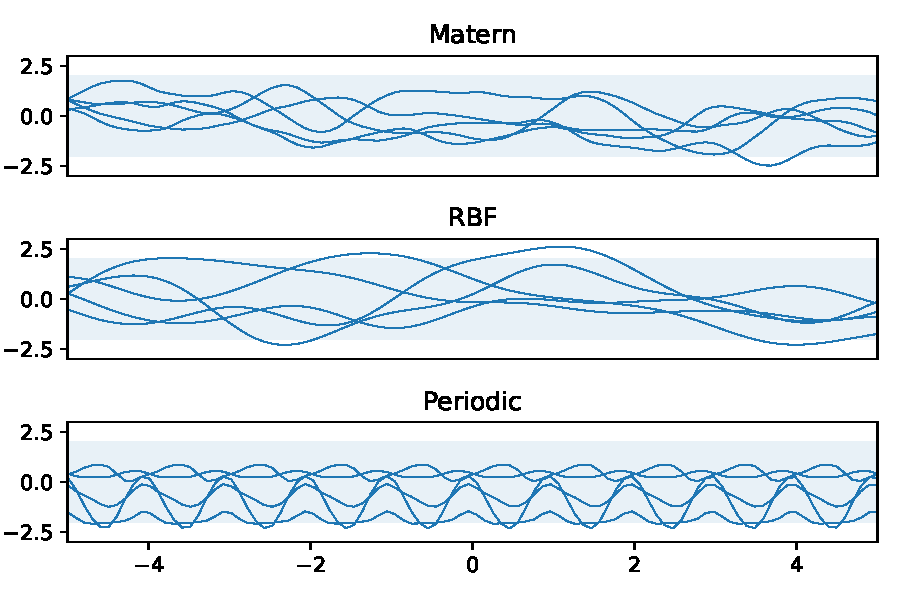
\includegraphics[width=0.8\linewidth]{../figures/prior.pdf}
  \centering
  \caption{Samples from different GP priors of RBF, Matérn and periodic kernel. We can see different kernels enforce different prior on the GP and hence the different behaviours (periodic, smoothness etc.) of the function sample.}
  \label{fig:prior}
\end{figure}

Now we intend to fit a GP to a dataset where the underlying function is $y=(x+x^2)\sin(x)$, arbitrarily defined for demonstration purpose.
We randomly sampled five points and the fit is as shown below in figure \ref{fig:posterior}.
We also sampled 10 posteriors.

\begin{figure}[H] 
  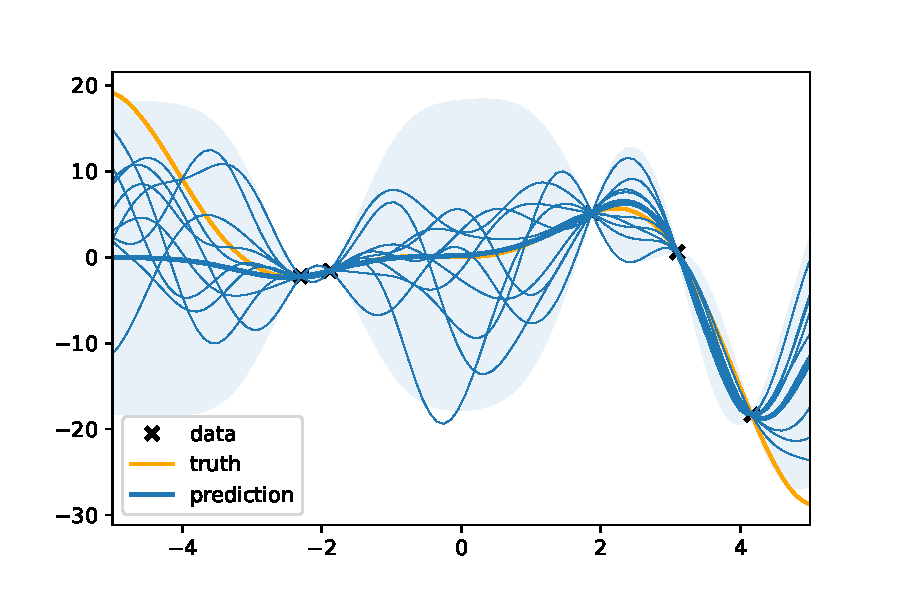
\includegraphics[width=0.8\linewidth]{../figures/posterior.pdf}
  \centering
  \caption{GP fit of the function $f=(x+x^2)\sin(x)$ with posterior samples, light shaded blue indicates 95\% credible interval. We can see that away from data, the GP is more uncertain.}
  \label{fig:posterior}
\end{figure}

We can see the function has low uncertainity around the data points and fall back to the GP prior (RBF in this case) away from the data.

\subsection{GPflow}
While we can in principle build our own GP objects using linear algebra and statistical libraries, such as Numpy, Scipy, from scratch, it is better to avoid errors and improve development speed by using a well-tested, robust and efficient library called GPflow, which will be used throughout the project (\cite{GPflow2017})\footnote[1]{The codes can be found in \url{https://github.com/charlielao/dynamical\_system\_invariance\_project}}.
It is a Python library built on TensorFlow to allow efficient and fast computation on GPUs to do GP inferences.
A particular powerful feature is that it allows atuomatic tuning of hyperparameter such as lengthscales and variance of a kernel by computing the gradient (using automatic differentiation feature of Tensorflow) and perform optimisation.
In later sections, when we will need to optimise more parameters than aforementioned ones with respect to maginal likelihood objective, the library will be proved to be very useful.

\section{Dynamical Systems}
Dynamical systems describe the evolution of a system in time, and can be broadly classified to two catergories: differential equations and difference equations, with the former being continous time and the latter being discrete time (\cite{strogatz_2019}). 
Here, we will illustrate the theory and notation using the continous time (differential equation) description.
There are many real world systems that can be modelled by a dynamical system; for example a huge class of problems in engineering and physics or biological processes. 
A simple example, which will also be explored later, is a damped harmonic oscillator, with equation of motion
\begin{equation}
m\frac{d^2x}{dt^2}+b\frac{dx}{dt}+kx=0,
\label{equ:damped}
\end{equation}
where $m, k, b$ are constants that depend on the setup and $x$ is the displacement of the mass.
In general an $n^{th}$ degree differential equations can be written as 
$$
\frac{d^{n} x}{d t^{n}}=F\left(t, x, \frac{d x}{d t}, \ldots, \frac{d^{n-1} x}{d t^{n-1}}\right),
$$
where $F$ is just some function (\cite{glendinning_1994}) and we will need $n$ initial conditions to specify a solution for the differential equations.
We can also write $n^{th}$ degree ordinary differential equations (ODEs) as $n$ degree one coupled ODEs \citep{strogatz_2019}. 
For example, we can rewrite equation \ref{equ:damped} as 
$$
\begin{cases}
  \frac{dx}{dt} = v\\
  \frac{dv}{dt} = \frac{-bv-kx}{m}\\
\end{cases}
$$
More generally, we can write 
$$
\begin{cases}
  \dot{x}_1=f_1(x_1, \dots, x_n)\\ 
  \vdots\\
  \dot{x}_n=f_n(x_1, \dots, x_n)\\ 
\end{cases}
$$

We can then visualise the state of the system specified by the $n$ variables, $x_1 \dots x_n$ in the phase space, and this system will evolve by moving in the phase space as time progresses. 
For instance, the damped oscillator is of degree 2 so there will be two variables describing its evolution, which in this case will be $x$ and $\frac{dx}{dt}=\dot{x}$, which is the displacement as well as velocity.
Another example would be a naive model describing exponential growth of a organism, such as bacteria population in a petri dish
$$
\dot{x}=rx,
$$
and this time it is one-dimensional with the phase variable being the population number, with $r$ again being a constant.
Another important concept is linearity and nonlinearity, which is referring to the $f_1, \dots ,f_n$ above.
If they depend on $x_1 \dots x_n$ linearly, then the system is linear, else it would be nonlinear.
Other examples of dynamical systems include predator-prey dynamics, planetry evolution, and many biological processes, such as drug treatments.
The systems discussed in the report include simple harmonic oscillators and single as well as double pendulums.



\section{Symmetry and Invariances}
Invariances are functions of the phase variables of a dynamical system that are unchanged throughout the evolution of the system over time. 
An example would be from physics, the conservation of energy, that energy will remain unchanged or constant throught out the trajectories of the system.
This is related to the symmetry under time translation.
There are other types of symmetry, such as translational symmetry, rotational symmetry, permutation symmetry, which are widely explored in geometric deep learning literature \cite{Bronstein2017}. 
More formally, we can describe symmetry using a little group theory.
Refering to \cite{Kondor2008}, we have symmetries and associated invariance if we have a symmetry group $G$ acting on $\mathcal{X}$, the input space, by $x\mapsto T_g(x)$ for $g\in G$, where $T$ is some transformation function parameterised by $g$. 
Then we should have $f(T_g(x))=f(x)$ for any function $f$, in other words, invariant under symmetry transformation.
For instance, if it is a rotational symmetric group then we will have $T$ corresponds to the rotation transformation of angle $g$, and we expect $f$ to be invariant under rotation.
In dynamical system, it has a slightly different interpretation.
From \cite{marsden_sirovich_antman_2008}, in this description of dynamical system, we consider a generator $\mathcal{L}$, which is an operator that generates the evolution of some function quantity that depends on the phase variables over time.
If we have the ODE $\frac{dx}{dt}=f$; then \begin{equation}\mathcal{L}[E]=\frac{dE}{dt}=f(x)\cdot \nabla_x E(x),\label{equ:LE}\end{equation} followed by simple chain rule, where $E$ is some function of the phase.
If we would like $E$ to be the conserved invariant quantity, we would then require $\mathcal{L}[E]=0$. 
This will then define what we mean by invariance in the context of dynamical system: some quantity depending on the input that does not change along the evolution of the system.

At first sight, there seems no apparent symmetry involved that is obvious like the rotational symmetry case. 
Neverthless, in physics, there is a deeper connection between symmetry and invariance, namely the Noether's Theorem, which is rather involved in theoretical classical physics and interested readers can refer to \cite{lemos_2018}.
In plain words, every conservation law (invariance) is associated with an underlying symmetry.
For instance, conservation of momentum is obeyed when there is a spatial translation symmetry of the system. 
Similarly, rotational symmetry is associated with the conservation of angular momentum.
There are more abstract conservation law, such as conservation of electrical charge is related to Gauge symmetry.
Here the more relevant ones is the conservation of energy, which is related to the symmetry of the system under temporal translation, i.e. the quantity is unchanged as time passes.


\section{Related Work}
There are many existing literature in the field of learning invariance, prediction in dynamical systems, as well as physics based machine learning methods.
A summary of comparison is made in table \ref{tab:compare}.

\subsection{Physics Informed Machine Learning}
Many physics informed machine learning techniques exist as outlined in \cite{Cuomo2022, PIML}
For example, in Physics Informed Neural Network (PINN) from \cite{Raissi2019}, the authors embedded the functional form of partial differential equations (PDEs) that describe the physics of the problem into the loss function so that the neural network model assume the PDE; they also allow the parameters in the PDEs to be learnt. 
There are many variants of such as \cite{Qian2020}.
In \cite{Raissi2018}, it even uses a GP to model the evolution of the state by using the PDE form as a linear operator to evolve the GP; since the linear transform of GP is still a GP, we will get joint GP, then we can do inference.
However, they are restricted to known PDE expression and only learn the coefficients instead of learning the whole physics from scratch. 
Moreover, for nonlinear dynamics, it has to use a linear approximation for the method to work, which is very restrictive.
There are also versions of PINN that takes conservation of energy into account such as \cite{Jagtap2020}.
However, it still suffers from other problems described above.

\subsubsection{Energy Conserving Neural Networks}
There are other approaches like Hamiltonian Neural Network (HNN) \citep{HNN}, which enforces the law of Hamiltonian mechanics (\cite{lemos_2018}), a model in theortical physics, on the neural network.
As a result, HNN automatically conserves the Hamiltonian or almost equivalently, the energy.
The experiments and setup of this report roughly follows that of the HNN paper.
There are also variants originated from this, such as the more general Lagrangian Neural Network \citep{Cranmer2020} using another theoretical physics framework or other energy conserving nerual networks described in \cite{Zhong2021}.
However, due to their strong invariance enforcing nature, they often do not do very well with dissipative systems; 
\cite{DissipativeHNN} models the dissipative part explicitly resolves this problem.
Nevertheless, these systems can only work on a very specific types of dynamical system, namely the ones that follow Sympletic form, or more simply follows the Hamiltonian mechanics, which is only a small subset of all dynamical systems.
There are a lot more general dynamical systems that has some sort of invariance property that is not able to utilise these energy conserving neural networks.
Moreover, learnability of invariance is less involved here that they are able to learn the value of energy but not actually recover the form of physics. 

\subsubsection{Symbolic approach}
An alternative way to recover the law of physics from trajectory uses various forms of symbolic regression, such as \cite{Udrescu2020, Papastamatiou2022} or some form of graphical representation \cite{GraphSymbolicPhysics, flexiblePhysics}.
In \cite{Liu2021}, it even able to deduce functional form the conserved quantity (along with its symbolic form) from trajectory.
However, again these are very physics focused examples, and the symbolic representation is often involves brute force; but of course it improves interpretability over functional approximation solution.

\subsubsection{ODE approach}
We can also directly works on the ODE that describes the physics of the system not dissimliar to PINN. 
Neural ODE (\cite{NeuralODE}) is a great example of this; 
however, again it does not use any knowledge of the invariances and symmetries.
In \cite{Lim2022}, they claimed that while Neural ODE is flexible, without built-in inductive biases of energy conservation, the model tends to grow or shrink in energy over a long period of time.
Furthermore, due to the extremely flexible expressibility of neural network, the ODE it learnt may not be the true physical model; which demonstrates the importance of building in such inductive bias.  

\subsection{Symmetry and Invariance in Machine Learning}

\subsubsection{Learning Invariance using Marginal Likelihood}
This paper forms the basis of this project.
In \cite{Mark2017}, the authors propose learning the form of invariances of the problem by parameterising the symmetry and optimise them with respect to the marginal liklihood.
The main problem studied in the paper is the MNIST dataset, and that the symmetry under consideration is all form of affine transformation of the images, such as rotation, shear, translation; and the invariance in this case is the label of the digit. 
It suggests embedding the invariance in the model (GP in this case) as an alternative to data augementation.
The authors created a special kind of kernel for GP that respects the symmetry of the problem.
The results are very good compare to the baseline RBF kernel, and it also is able to recover the true paramertised invariance. 
The logical flow and procedure of investigation of this report follows closely on this paper. 
A related paper following that uses a neural network instead of GP is Van der Ouderaa and Van der Wilk (2022) using the same idea by optimising the marginal likelihood.

\subsubsection{Geometric Deep Learning}
Geometric deep learning proposed by \cite{Bronstein2017}, is a unifying framework that aims to explain the success of several popular neural network architecture. 
For example, Convolution Neural Network uses the translation symmetry embedded in natural images. 
Another example is Graph Neural Network utilises the permutation symmetry that the graphs is invariant under permutation.
Following this framework, multiple papers are proposed that aims to exploit further symmetry groups (5Gs Grids, Groups, Graphs, Geodesics, and Gauges).
These show that how powerful the inductive bias of symmetry and invariances are.

\subsection{GP in dynamical systems}
There are also a number of research work that use GP to predict dynamical system evolution.
One of them is the aforementioned \cite{Raissi2018}.
There is also \cite{Rath2020}, that utilise the Sympletic nature of Hamiltonian systems to directly predict the flowmaps of the system, which is similar to HNN.
There is also \cite{Heinonen2018}, that also uses GP to model the ODE models in a nonparametric manner; but again it does not use invariance, and is more like Neural ODE. 

\begin{table}[H]
    \centering
\begin{tabularx}{\linewidth}{c|LLL} 
    \hline
 Methods & Respect the physics laws & Recover the physics laws & Generalise to dynamical systems beyond physics  \\ 
    \hline
  ODE approach & X & O & O \\
  Symbolic approach & O & O & X \\
  Physics informed ML & O & X & X \\
  Energy conserving NN & O & X & X \\
  GP in dynamical system & X & O & O\\
  Our method & O & O & O\\
    \hline
\end{tabularx}
\caption{Comparing the capabilities of different existing approach to learning invariance in dynamical systems}
\label{tab:compare}
    \end{table}



\chapter{Invariance Kernel}
In this chapter we will start with general theoretical construction of invariance kernel given the knowledge of the invariance of the system.
Recall in section 2.1, differnt kernels assume differnt prior on the GP; we will therefore attempt to embed our invariance priors into the kernel so the GP respects the invariance.
We will then describe how we are able to accomdation dissiaptive systems.
Finally, we will demonstrate how we are able to learn invariances without any prior knowledge of the system.

\section{General Construction}
If we are given a dynamical system of dimension $d$ with variables $\mathbf{q}, \mathbf{p}$, where $\mathbf{q} = (q_1, q_2,\dots,q_d)$ is the vector of positional coordinates, and $\mathbf{p}=(p_1, p_2, \dots, p_d)$ is the vector of velocity coordinates of the states of the dynamical system.
We are interested to predict the future trajectories of the state of the system.
Therefore, we would like to know the time derivative of these coordinates so we can update them using an integrator (e.g. Euler, Runge-Kutta). 
These time derivatives are referred to as the \textbf{dynamics} of a dynamical system, which governs the evolution of the system, and is a function of the coordinates $\mathbf{q}$ and $\mathbf{p}$ (it could also be explicitly time dependent but that will be a straightforward generalisation, and so is not considered here). 

For our systems, we will denote the dynamics of $\mathbf{p}$ as $\frac{d\mathbf{p}}{dt}=\mathbf{a}(\mathbf{q}, \mathbf{p})$, and that of $\mathbf{q}$ as $\frac{d\mathbf{q}}{dt}=\mathbf{v}(\mathbf{q}, \mathbf{p})$.
Astute readers or someone with physics background would notice $p$ is related to the velocity, which in principle should be exactly equal to $v$; while this is true in physical dynamical system, the setup is generally applicable to non physical dynamical systems too, so that we will not use this knowledge. 

Once we have the dynamics, we can integrate up with respect to time using a numerical integrator to obtain the future trajectories. 
Notation wise, we will collect the two dynamics term and call them $$\mathbf{f(\mathbf{q}, \mathbf{p})}=\begin{pmatrix}
    \mathbf{a(\mathbf{q}, \mathbf{p})}\\\mathbf{v(\mathbf{q}, \mathbf{p})}
\end{pmatrix}$$
For simplicity of notation, the dependence on $\mathbf{q}, \mathbf{p}$ is now implicit. 

The goal is to learn the dynamics, so for the inference procedure, we choose to put GP priors on $\mathbf{f}$ so that $\mathbf{f}\sim\mathcal{GP}(m, K)$.
We will choose $m$ to be zero since there is no obvious prior knowledge for the mean function.
We will also assume $\mathbf{a}$ and $\mathbf{v}$ to be independent since there are no reason to assume otherwise. 
For the choice of kernel, we chose the standard smooth kernel, the squared exponential kernel, or RBF, and we denote this kernel to be $K_{RBF}$. 
We will also denote any set of points in the input space of length $n$ and dimension $d$ as $$X\equiv\begin{pmatrix}
    \mathbf{x}_1\\\mathbf{x}_2\\\vdots\\\mathbf{x}_n
\end{pmatrix}=\begin{pmatrix}
    q_{11}& q_{21} &\dots& q_{d1} & p_{11} & p_{21} & \dots & p_{d1} \\
    q_{12}& q_{22} &\dots& q_{d2} & p_{12} & p_{22} & \dots & p_{d2} \\
    \vdots &\vdots &\ddots &\vdots &\vdots &\vdots &\ddots &\vdots \\
    q_{1n}& q_{2n} &\dots& q_{dn} & p_{1n} & p_{2n} & \dots & p_{dn} \\
\end{pmatrix}.$$
Without loss of generality, we will choose to stack the dynamics vertically in $\mathbf{f}$; for example in a $d$-dimensional system, we have \begin{equation}\mathbf{f}(X)=\begin{pmatrix}
    a_1(\mathbf{x}_1)\\
    \vdots\\
    a_1(\mathbf{x}_n)\\
    \vdots\\
    a_d(\mathbf{x}_1)\\
    \vdots\\
    a_d(\mathbf{x}_n)\\
    v_1(\mathbf{x}_1)\\
    \vdots\\
    v_1(\mathbf{x}_n)\\
    \vdots\\
    v_d(\mathbf{x}_1)\\
    \vdots\\
    v_d(\mathbf{x}_n)\\
\end{pmatrix}\label{equ:stacked}\end{equation}
For our naive independent RBF GP prior, we will finally have the covariance matrix K (kernel) being a block diagonal 
\begin{CentreLongEquation}
$$
K=\mathrm{Cov}(\mathbf{f}(X), \mathbf{f}(X'))=\begin{pmatrix}
    K_{RBF,a_1}(X,X') & \dots  & \dots          & \dots         & 0\\
    \vdots        & \ddots & \dots          & \ddots        & \vdots\\
    0             & \dots  & K_{RBF,a_d}(X,X')  & \dots         & 0 \\
    \vdots        & \ddots & \vdots         & K_{RBF,v_1}(X,X') & \vdots \\
    0             & \dots  & 0              & \dots         & K_{RBF,v_d}(X,X')\\
\end{pmatrix},
$$
\end{CentreLongEquation}
with all the off diagonal terms being zero block matrixes because of the independence assumption between dynamics.
Note that each $K_{RBF}$ is independent from one another with independent hyperparameters.
This naive kernel will be our baseline to be compared to throughout the whole project.
This is essentially a GP model without any knowledge of the invariance, and simply treating the dynamics as targets like standard GP regression tasks we considered in section 2.1 and equation \ref{equ:joint_gp_noise}.

Now we can start considering the invariance. 
If we assume the invariance constraints has to hold throughout the input phase space $\mathbb{R}^{2d}$, then we can condition the baseline GP on a grid of points covering the input space, which we referred to invariance points, $X_L$, where the invariance constraints hold. 
We denote $\ell$ as the number of invariance points, and we will call the invariance constraints $\mathcal{L}[E]$ as described in section 2.3.

The form of $\mathcal{L}[E]$ will depend on the system as well as $X_{L}$, and examples will be given in chapter 3 to make it clear.
Since the conservation of energy, $E$, is one of the most common invariance in physical systems, we will focus on making use of this constraint.
Therefore, we have $E=\text{energy}.$
We can see the invariance constraints will always be a linear function on the dynamics $\mathbf{f}=\begin{pmatrix}
  \mathbf{a} \\ \mathbf{v}
\end{pmatrix}$ almost by definition because of chain rule as shown in the next paragraph.

We have $\text{energy}=E(\mathbf{\theta}, \mathbf{p}, \mathbf{q})$, where $\mathbf{\theta}$ are constants that parameterised the energy function, like mass or gravity.
Then refering back to equation \ref{equ:LE}, we have 
\begin{equation}
\mathcal{L}[E] = \frac{dE}{dt}=\sum_{i=1}^d \frac{\partial E}{\partial p_i} \frac{\partial p_i}{\partial t}+ \sum_{i=1}^d\frac{\partial E}{\partial q_i}\frac{\partial q_i}{\partial t} =\sum_{i=1}^d \frac{\partial E}{\partial p_i} a_i(\mathbf{p,q}) + \sum_{i=1}^d\frac{\partial E}{\partial q_i} v_i(\mathbf{p,q})
\label{equ:invariance_equation}
\end{equation}
We can therefore see it is always a linear combination of dynamics with coefficients independent of dynamics.
As a result, $\mathcal{L}[E]$ can be seen to be a linear transformation of $\mathbf{f}$, and now we call this transformation operator $L$ acting on the dynamics, which will be a function of $\mathbf{p}, \mathbf{q}$ and $\mathbf{\theta}$.
If we apply this linear transformation $L$ on $\mathbf{f}(X_L)$, $L[\mathbf{f}(X_L)]$ will again be a GP with a transformed kernel because of the property of multivariable normal distribution.
$$
\text{if } x\sim\mathcal{N}(0, K);\ Ax\sim\mathcal{N}(0, AKA^T),
$$
where A is some linear operator.
Therefore, building on our baseline GP model, we have joint distribution
\begin{equation}
\begin{pmatrix}
\mathbf{f}(X)\\L[\mathbf{f}(X_L)]
\end{pmatrix}
\sim\mathcal{N}
\left(\begin{pmatrix}\mathbf{0}_{2nd}\\\mathbf{0}_{\ell}\end{pmatrix}, \begin{pmatrix}
    K & LK \\
    KL^T & LKL^T\\
\end{pmatrix}\right)
\label{equ:invariance_joint}  
\end{equation}
To impose the constraints on the invariance points, we then condition the first row on the second row being zero using equation \ref{equ:normal_condtion} to obtain
\begin{equation}
  \mathbf{f}(X)|L[\mathbf{f}(X_L)]=0 \sim \mathcal{N} \left(\mathbf{0}_{2nd}, \begin{pmatrix}
    K-LK(LKL^T)^{-1}KL^T
  \end{pmatrix}\right)
  \label{equ:invariance_condition}
\end{equation}
The kernel in equation \ref{equ:invariance_condition} will then be our invariance kernel.

\section{Damped System}
Up to now, we have considered a perfect system, i.e. ideal world without frictions and the conservation of energy is completely obeyed such that $L[\mathbf{f}(X_L)]=0$ exactly.
However, in a real system, there will be dissipation where energy is lost in the form of heat etc.  
For example, in equation \ref{equ:damped}, the frictional force enters through the $b\frac{dx}{dt}$ term that makes the system loss energy to the surrounding as heat.  
Therefore, to model that, we need to allow "approximate" invariance, such that the invariance $L[\mathbf{f}(X_L)]$ is noisy and not always exactly equal to zero, i.e. soft invariance.
To account for that, in a similar spirit to when we add noise to the underlying latent GP to represent noise signal in equation \ref{equ:joint_gp_noise}, such that we have $K+\sigma_n^2 \mathbb{I}$;
we will therefore add a noise to the invariance evaluation so that we have $L[\mathbf{f}(X_L)]=\epsilon$, where $\epsilon\sim\mathcal{N}(m_L, \sigma_L^2)$.
Therefore, instead of equation \ref{equ:invariance_joint}, we will have 
$$
\begin{pmatrix}
\mathbf{f}(X)\\L[\mathbf{f}(X_L)]
\end{pmatrix}
\sim\mathcal{N}
\left(\begin{pmatrix}\mathbf{0}_{2nd}\\\mathbf{m}_{\ell}\end{pmatrix}, \begin{pmatrix}
    K & LK \\
    KL^T & LKL^T+\sigma_L^2\mathbb{I}\\
\end{pmatrix}\right),
$$
Again, the white noise will only affect the variance part of $L[\mathbf{f}(X_L)]$ and not its covariance with $\mathbf{f}(X)$.
We will then able to do the conditioning according to equation \ref{equ:normal_condtion} again and obtain
\begin{equation}
  \mathbf{f}(X)|L[\mathbf{f}(X_L)]=0 \sim \mathcal{N} \left(-LK(LKL^T+\sigma^2_L\mathbb{I})^{-1}\mathbf{m}_\ell, \begin{pmatrix}
    K-LK(LKL^T+\sigma^2_L\mathbb{I})^{-1}KL^T
  \end{pmatrix}\right)
\label{equ:damped_invariance}
\end{equation}
Here, the parameters $\mathbf{m}_L$ and $\sigma^2_L$ will be learnt by optimising marginal likelihood. 
The reason we allow the noise to have a non-zero mean is that we know that the energy can only decrease so that $\frac{dE}{dt}\equiv L[\mathbf{f}(X_L)] \le 0 $, so the deviation of invariance from zero is not symmetrical between positive and negative as a zero mean Gaussian noise would; we therefore introduce a learnable negative mean to accounts for that.  
The idea of introducing this soft invariance noise is that hopefully this relaxation of the contrains of invariance will allow the model to use some information of invariance to do prediction and at the same time not strictly enforcing it, which would have lead to poor performance. 
We will also use an alternative method to model the dissipative dynamics of the system using latent variables as shown in the section 3.4. 


\section{Learning Invariance}
Previously, we have assumed the knowledge of the dynamics equation from Newton's Law, which has allowed us to derive the energy, $E$ and the invariance linear transformation $L$ accordingly. 
However, for the kernel to be useful in real life, we cannot assume the equations of the system beforehand, since if we have the knowledge, then we can just use a numerical ODE integrator to obtain the trajectories. 
Therefore, we should find a way for the system to learn the form of invariance from data directly.
The way we chose to do so is to parameterise our invariance function and allow the system to learn the coefficients of the paramerterisation by maximising the log marginal likelihood.
(Interestingly, even if we specify the form of invariance, we would still not completely solve the system since there are still lots of degree of freedom left as will be illustrated in the next chapter.) 

\subsection{One-dimensional system}
There are many different ways to paramerterise an unknown function, including but not limited to Fourier representation, neural networks, wavelets, splines.
As the problems are relatively bounded, we chose to use polynomial basis to paramerterise the unknown function $\mathcal{L}[E]\equiv L[\mathbf{f}]$.
In other words, we will be paramerterising the $\frac{\partial E}{\partial p_i}$ and $\frac{\partial E}{\partial q_i}$ term in equation \ref{equ:LE}.
Using polynomial basis is very efficient in our cases since there will only be a few coefficents to learn.
On the other hand, if we use much more expressive splines or neural networks, we will have many more parameters to optimise, and can even easily lead to overfitting.
Not using Fourier series is because we know there can be many linear functions, and we may need a large number of Fourier series expansion to accomdate that; so the most natural choice for our task is to use polynomials.

In one-dimensional cases, for our examples, they are simple enough so that $L[\mathbf{f}]$ is separable so that we have a function of $p$ only, $f(p)$ and a different function of $q$ only, $g(q)$, such that $L[\mathbf{f}]=f(p)a+g(q)v$ so that $f, g$ can be learnt seperately with no mixing between $p$ and $q$.
In the one-dimensional SHM case, $f(p)=mp$ and $g(q)=kq$.
For simple pendulum, we have $f(p)=\ell p$ and $g(q)=\sin q$.
We will therefore set $$f(p)=\sum_{i=0}^{n_f}c_{f,i}p^i,\ g(q)=\sum_{i=0}^{n_g}c_{g,i}q^i,$$
where $c_{f,i}, c_{g,i}$ are the parameters we will optimise based on marginal likelihood and we will evaluate different degree of polynomial $n_f, n_g$ and see which combinations produce the highest marginal likelihood. 

\subsection{Two-dimensional system}
In two-dimensions, things are a bit more complicated. 
For example, it is very clear that in double pendulum shown in chapter 3, the invariance constraints is not seperable.
Instead, we need to consider all combinations of polynomials; i.e. multivariate polynomial.
Therefore, for two-dimensions we have $L(\mathbf{f})=f_1(p_1, p_2, q_1, q_2)a_1+f_2(p_1, p_2, q_1, q_2)a_2+g_1(p_1, p_2, q_1, q_2)v_1+g_2(p_1, p_2, q_1, q_2)v_2$.
We will paramertise each of $f_1, f_2, g_1, g_2$ with $$\sum_{i,j,k,l=0}^{n}c_{ijkl}p_1^ip_2^jq_1^kq_2^l$$
Therefore, there will be many more coefficients to be optimised.
We can calculate the number by using the combination with replacement formula
$$
C^R(n, r) = \frac{(n+r-1)!}{r!(n-1)!},
$$
where $n$ is the number of choices (4 in this case) and $r$ is the number we are choosing.
For example, if we wish to have a cubic polynomial, then we would require $\frac{(4+3-1)!}{3!(4-1)!}+\frac{(4+2-1)!}{2!(4-1)!}+\frac{(4+1-1)!}{1!(4-1)!}+\frac{(4+0-1)!}{0!(4-1)!}=35$ parameters for each polynomial so we would require $35\times 4=140$ parameters in total.

\section{Partially Observed System}
Partially observed data can be very common in dynamical system.
With examples of physical system, we can imagine not observing $p$ and only observe $q$ (of course we do not possess the knowledge that $\dot{q}=p$).
This will correpond to just observing the trajectory of a particle but has no information about the time and hence we cannot deduce velocity.
If we have a two-dimensional system, we might only observe one set of dimension due to data recording mechanism, or perhaps some situation where we project three-dimensional objects on to the wall and we can only observe the two-dimensional shadows.
In a more general sense, we can imagine if we have a system with unquantifiable friction (without prior knowledge).
We may not be able to write down the form of friction analytically due to complex interaction of the system with the enviroment (i.e. not simply a damped system as shown in equation \ref{equ:damped}, where it is analytical).
Nevertheless, the law of physics and conservation of energy will still hold in the broad sense; 
in other words, if we take into account of every single force of the interactions (including the enviroment), the total energy will be conserved so the invariance holds. 
For example, in the case of frictional forces, they arise because of the electric-magnetic forces between particles and the surface of the enviroment.
If we take into account of the particles on the surface and their interactions with the particles in our system, the energy will again be conserved. 
In practice, we can only observe the system so that the rest of the physics (interaction with the enviroment) is not observed, so it is again a partially observed problem.

To address this issue, we can use a latent variable model. 
The idea is to model the unobserved variable as a latent variable $z$ and its associated time derivative as dynamics $\dot{z}$.
For example, if we only observe $q$ in an one-dimensional system, then we can set $z=p$, a latent variable. 
Then the dynamics $f$ will include the $\dot{z}$ term, which is equivalent to $a$ if it is observed. 
In the case of two-dimensional system, where we do not observe the $p$ nor $q$ of one dimension, we will then have two latent variables $z_1, z_2$ and their associated dynamics.
We can then use the invariance condition as before to constrain the distribution of the latent variables and does inference on it using inference scheme such as Markov Chain Monte Carlo or Variational Inference since we need to integrate out the latent variables, and is often intractable.

In this report, we will focus on one particular problem: the damping case.
Here, we do not have missing inputs; instead, we have missing dynamics that accounts for the dissipative forces. 
Therefore, we invent the latent variable $z$ to represent the dissipative effect.
Now, instead of the invariance in equation \ref{equ:invariance_equation} being equal to zero, $\frac{dE}{dt}\equiv\mathcal{L}[E]=0$, we have $\frac{dE}{dt}+z=0,$ so that now we have 
\begin{equation}
\mathcal{L}[E] + z = \frac{dE}{dt} + z =\sum_{i=1}^d \frac{\partial E}{\partial p_i} \frac{\partial p_i}{\partial t}+ \sum_{i=1}^d\frac{\partial E}{\partial q_i}\frac{\partial q_i}{\partial t} + z = \sum_{i=1}^d \frac{\partial E}{\partial p_i} a_i + \sum_{i=1}^d\frac{\partial E}{\partial q_i} v_i + z,
\label{equ:LEplusZ}
\end{equation}
which is therefore the a linear transformation on an augmented dynamics $\mathbf{f_\gamma}=\begin{pmatrix}
  \mathbf{f}\\z
\end{pmatrix},$
and we will define this new linear transformation as $L_\gamma$, which operates on $\mathbf{f_\gamma}.$
Effectively, we treat $z$ as dynamics with equal footing with $\mathbf{a}$ and $\mathbf{v}$.
Following this argument, in a similar fashion as section 3.1, we will again put an GP prior on $z$ with RBF kernel, that is independent from $\mathbf{f}$.
Now instead of equation \ref{equ:invariance_joint}, we have 
\begin{equation}
\begin{pmatrix}
\begin{pmatrix}\mathbf{f}(X)\\ z(X)\end{pmatrix}\\L_\gamma[\mathbf{f}(X_L), z(X_L)]
\end{pmatrix}
\sim\mathcal{N}
\left(\begin{pmatrix}\mathbf{0}_{3nd}\\\mathbf{0}_{\ell}\end{pmatrix}, \begin{pmatrix}
    K & L_\gamma K \\
    KL_\gamma^T & L_\gamma KL_\gamma^T\\
\end{pmatrix}\right),
\label{equ:joint_withZ}
\end{equation}
where now 
$$
K = \begin{pmatrix}
  K_f & 0 \\
  0 & K_z\\
\end{pmatrix},
$$
Finally, using the normal conditional formula \ref{equ:normal_condtion}, we have 
\begin{equation}
  \begin{pmatrix}\mathbf{f}(X) \\ z(X) \end{pmatrix}|L_\gamma[\mathbf{f}(X_L), z(X_L)]=0 \sim \mathcal{N} \left(\mathbf{0}_{3nd}, \begin{pmatrix}
    K-L_\gamma K(L_\gamma KL_\gamma^T)^{-1}KL_\gamma^T
  \end{pmatrix}\right)
  \label{equ:invariance_condition_withZ}
\end{equation}

As we only have the data for $\mathbf{f}(X)$, we will need to marginalise the joint distribution between $\mathbf{f}$ and $z$ by integrating over all possible $z$, $\int p(\mathbf{f},z) dz$.
Fortunately, for multivariate normal distribution, if we have
$$
\begin{pmatrix}
  x \\ y
\end{pmatrix}
\sim\mathcal{N}
\left(
  \begin{pmatrix}
    m_x \\ m_y 
  \end{pmatrix},
\begin{pmatrix}
  V_{xx} & V_{xy} \\ V_{yx} & V_{yy} \\
\end{pmatrix}
\right),
$$
then 
$$
x\sim\mathcal{N}(m_x, V_{xx}).
$$
We therefore have 
$$
\mathbf{f}(X)|L_\gamma[\mathbf{f}(X_L), z(X_L)]=0 \sim \mathcal{N}(\mathbf{0}_{2nd}, [K-L_\gamma K(L_\gamma KL_\gamma^T)^{-1}KL_\gamma^T]_{[0:2nd, 0:2nd]}),
$$
where for a matrix $M$, $M_{[0:r,0:c]}$ is a submatrix of $M$ equal to the first $r$ rows and first $c$ columns of the $M$ (zero indexed).
At the same time, we are able to get the posterior of $z$ in the same inference procedure. 
If we denote 
$$
K-L_\gamma K(L_\gamma KL_\gamma^T)^{-1}KL_\gamma^T \equiv \begin{pmatrix}
  V_{ff} & V_{fz} \\ V_{zf} & V_{zz} \\
\end{pmatrix},
$$
where $V_ff$ is the submatrix of the full covariance matrix corresponds to variance of $\mathbf{f}(X)$ (i.e. the first $2nd$ rows and $2nd$ columns as before), the rest are defined accordingly.  
Then using the normal condition formula \ref{equ:normal_condtion} once again, 
$$
z(X)|\mathbf{f}(X)=Y, L_\gamma[\mathbf{f}(X_L), z(X_L)]=0
\sim\mathcal{N}
(V_{zf}V_{ff}^{-1}Y,\ V_zz-V_{zf}V_{ff}^{-1}V_{fz}),
$$
where $Y$ is the data for the observed dynamics.

\chapter{Experiments}
\section{Data Generation}
To generate the data, we use a Runge-Kutta integrator to generate trajectories using the equation of motions for each problem. 
We also added some small Gaussian noise $10^{-8}$ to the dynamics (the time derivative of variables) when integrating to reflect the real world better as well as stablising the integrator.
Since we aim to predict the value of dynamics at any point in the input space, we use the dynamics as targets, $Y$. 
This is obtained by combining forward and backward finite difference (midpoint method) to compute the gradient. 
To illustate, $f'(x_1)=\frac{f(x_2)-f(x_0)}{2h}$, where $h$ is the spacing between $x_0, x_1$ and $x_1, x_2$ and $f'(x_1)$ is the derivative evaluated at $x_1$.
We also choose the time step to be $0.01$ to ensure sufficient accuracy for the integrator.
For training data, $X$, we choose a few random starting point within a range (datails depends on the task as described later) in the input space and generate data from there for a number of timesteps (again, tasks specific). 
To assess the performance, we generate the test set using the same input range, we will pick ten different starting points and then average the result.

\section{Evaluation Method}
We will mainly use the mean squared error (MSE) between the trajectory prediction and ground truth as our evaluation metrics. 
We also illustrate the amount of energy (using the exact expression) along the trajectory to demonstrate that invariance is obeyed.
For learning the invariance in one-dimensional case, we can also further compare the true invariance and the learnt invariance up to a multiplicative constant.
However, it is not possible to visualise in two-dimensional cases so we will simply assess the conservation of energy (invariance) performance.

\section{Implementation Technicalities}
We will need to add jitter, a diagonal matrix of small value, to the $LKL^T$ matrix in equation \ref{equ:invariance_condition}.
This is due to the fact that we need the invert it and it will be more stable numerically if we add a little bit of jitter in the range of $10^{-6}$ to $10^{-4}$.
As this is a common practice, its effect on the model will be in the Appendix for intereseted readers.
Similarly, for stability, when backpropagating to optimise the hyperparameters with respect to marginal likelihood, we need to narrow the range of search such that the value is more reasonable.
It is particularly important in our dynamical systems since, for example, in SHM the equation of motion is $a=-q$ and $v=p$, so that is will be a flat two-dimensional plane extends to infinity;
as a result, if the GP successfully recover the true invariance, the lengthscales of certain dimensions will be very large or $\infty$ (a property of ARD kernel, essentially able to set a dimension to constant), and it would not affect the performance a lot if we limit the lengthscales for a much smaller value to avoid instability.
Therefore, here I would set the range of both lengthscales and variable to be around the two to three times the maximum range possible.
For example, if we have maximum range of $\pm 2$, my upper bound for search is set to $10$ and lower bound is $10^{-6}$.

\subsection*{Invariance points $X_L$}
In low dimensions, we could simply allow $X_L$ to be a evenly spaced grid in the input space, and we will call the number of points in each dimension the \textbf{invariance density}.
So that if we have an invariance density of $40$, it means $X_L$ will contain $1600$ points in one-dimensional cases. 
However, conditioning on a grid of invariance points is simply not scalable in high dimensions. 
If we have an invariance density of 10 in a $\pm 5$ range for two-dimensional SHM (spacing of 1), then we will have 10000 points. 
We can easily run out of memory and also taking the matrix inverse are very difficult and time consuming.
As a result, to make the approach scalable to high dimensional space, we will use the idea of local invariance. 

The idea is straightforward, we simply sample uniformly (20-80 points) in the local region around the training and testing points and set them as $X_L$ (we choose a torus shape around the data points so that we will not have invariance points too close to the data points, making it unstable).
Note that we only sampled once, so that the same local grid will be centred on every training and testing points; this is done to remove the randomness for stability and dependence on the data.
We will still have the global grid invariance points as before (with smaller invariance density) so that we can still impose some degree of invariance if the test points are very far from the training points.
This works on the assumption that only the region around testing points will be the most important to predict in terms of conditioning; and to use the same kernel expression, we also have to condition on the region around training points, which is also important to help maximising the marginal likelihood objective when we are learning the invariance function.
Another evidence that supports the use of local invariance, which have much fewer points than using a grid, is demonstrated below where we show that there is a diminishing return in increasing the number of invariance points so that actually not that many invariance points is needed to achieve a good performance. 

\section{One-dimensional System}
\subsection{Linear SHM}
We will first examine one of the most simple dynamical system, an one-dimensional simple harmonic motion (SHM). 
An example would be a mass spring system as shown in figure \ref{fig:shm_diagram} with mass $m$ and spring constant $k$, and an example trajectory is shown in figure \ref{fig:shm_trajectory}. 
The $q$ is the displacement of the block from its origin, and $p$ would be the instanteous velocity.

\begin{figure}[H]
        \centering
        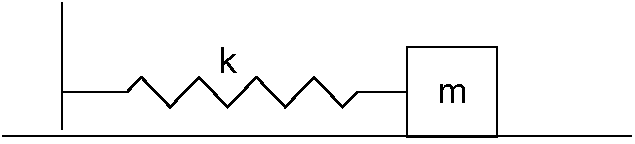
\includegraphics[width=0.8\linewidth]{../figures/shm.pdf}
        \caption{A simple mass spring system where after the mass is displaced, it will undergo simple harmonic oscillation.}
        \label{fig:shm_diagram}
\end{figure}

The equation of motion of the system is given by $$m\frac{d^2q}{dt^2}=-kq,$$
with the analytical solution of the form $q=A\sin(\omega_0t+\phi),$ where $\omega_0=\frac{k}{m}$ and $A, \phi$ depends on the initial condition, which dictates the amplitude and phase of the motion respectively. 
In this case, we have dynamics of the form 
$$
\mathbf{f}(\mathbf{x})=\begin{pmatrix}
    a(\mathbf{x})\\
    v(\mathbf{x})\\
\end{pmatrix}
$$

\begin{figure}[H] 
  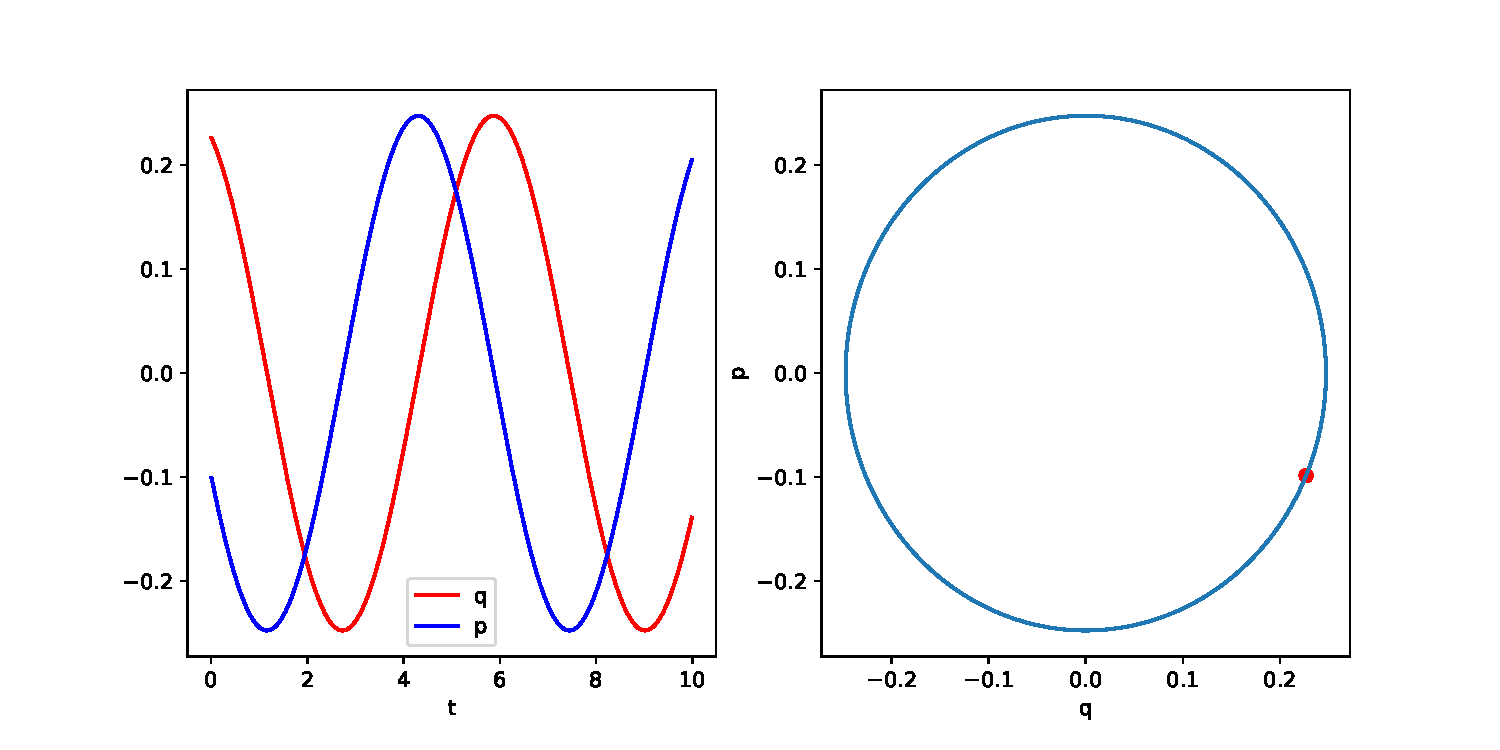
\includegraphics[width=0.7\linewidth]{../codes/figures/shm_trajectory_1D.pdf}
  \centering
  \caption{Example trajectory of SHM where we can see the trajectory is a perfect circle.}
  \label{fig:shm_trajectory}
\end{figure}

We also have the energy, $E=\frac{mp^2}{2}+\frac{kq^2}{2}.$
Therefore, to obtain our invariance $L$, we use the conservation of energy $\frac{dE}{dt}=0$ so from equation \ref{equ:invariance_equation}, we finally have $$L[\mathbf{f}]=mpa+kqv=0$$
While $L$ is not able to be put into a matrix form using our stacked representation in equation \ref{equ:stacked} (since the dimension would not match), it is a linear operator as shown below. 
If we have $$X_L\equiv\begin{pmatrix}
    \mathbf{x}_{L,1}\\
    \vdots\\
    \mathbf{x}_{L,\ell}\\
\end{pmatrix}=\begin{pmatrix}
    q_{L,1} & p_{L,1}\\
    \vdots & \vdots \\
    q_{L,\ell} & p_{L,\ell}\\
\end{pmatrix}\equiv\begin{pmatrix}
    \vdots & \vdots\\
    q_L & p_L\\
    \vdots & \vdots\\
\end{pmatrix},$$
then we have for either the known form of invariance in the middle or the paramerterised version on the right:
$$
L([\mathbf{f}(X_L)]) = \begin{pmatrix}
   mp_{L,1}a(q_{L,1},p_{L,1}) + kq_{L,1}v(q_{L,1},p_{L,1})\\ 
   \vdots \\
   mp_{L,\ell}a(q_{L,\ell},p_{L,\ell}) + kq_{L,\ell}v(q_{L,\ell},p_{L,\ell})\\ 
\end{pmatrix},
$$
which can be readily checked to be linear.
The requirement of an operator $T$ is said to be linear if 
$$
\begin{cases}
  T(x+y) = T(x)+T(y)\\
  T(\alpha x) = \alpha T(x)
\end{cases},
$$
where $\alpha$ is some constants, and $x, y$ are some inputs.

As explained in section 3.1, we will then apply this linear transform on our original GP prior to produce a joint distribution in the form of equation \ref{equ:invariance_joint}:
\begin{equation}
\begin{pmatrix}
    \mathbf{f}(X)\\
    L([\mathbf{f}(X_L)])\\
\end{pmatrix}
\sim\mathcal{N}
\left(\begin{pmatrix}
    0_{2n}\\0_{\ell}
\end{pmatrix},\begin{pmatrix}
   A & B \\
   C & D\\ 
\end{pmatrix}\right),
\label{equ:jointABCD}
\end{equation}
where
\begin{equation}
\begin{gathered}
A=K(X,X), B=\begin{pmatrix}
    K_{RBF,a}(X, X_L) \\ K_{RBF,v}(X, X_L) \\
\end{pmatrix}\odot \begin{pmatrix}
    mP_L \\ kQ_L
\end{pmatrix}, C=B^T,\\ D=K_{RBF,a}(X_L, X_L)\odot m^2(p_L\otimes p_L) + K_{RBF,v}(X_L, X_L)\odot k^2(q_L\otimes q_L),
\end{gathered}
\label{equ:ABCD}
\end{equation}
where $\odot$ is the elementwise product and $\otimes$ is the outer product so that 
$$
P_L=\begin{pmatrix}
  p_{L,1}  & \dots & p_{L,\ell}  \\
  \vdots & \text{repeats n rows} &  \vdots\\
  p_{L,1}  & \dots & p_{L,\ell}  \\
\end{pmatrix},
Q_L=\begin{pmatrix}
  q_{L,1}  & \dots & q_{L,\ell}  \\
  \vdots & \text{reqeats n rows} &  \vdots\\
  q_{L,1}  & \dots & q_{L,\ell}  \\
\end{pmatrix}
$$
and we have 
$$
p_L\otimes p_L=\begin{pmatrix}
  p_{L,1}^2 & p_{L,1}p_{L,2} & \dots & p_{L,1}p_{L,\ell} \\
  \vdots & \vdots & \vdots & \vdots \\
  p_{L,\ell}p_{L,1} & p_{L,\ell}p_{L,2} & \dots & p_{L,\ell}^2 \\
\end{pmatrix},
q_L\otimes q_L=\begin{pmatrix}
  q_{L,1}^2 & q_{L,1}q_{L,2} & \dots & q_{L,1}q_{L,\ell} \\
  \vdots & \vdots & \vdots & \vdots \\
  q_{L,\ell}q_{L,1} & q_{L,\ell}q_{L,2} & \dots & q_{L,\ell}^2 \\
\end{pmatrix},
$$ 
These matrix expressions are derived as follows by computing the covariance manually. 
For $B$, we wish to calculate 

\begin{align*}
B_{ij} &= \mathrm{Cov}(\mathbf{f}(X), L[\mathbf{f}(X_L)])_{ij} \\
       &= \mathrm{Cov}(\mathbf{f}(X)_i, L[\mathbf{f}(X_L)]_j) \\ 
       &= \begin{cases}
        \mathrm{Cov}(a(q_i, p_i), mp_{L,j}a(q_{L,j},p_{L,j}) + kq_{L,j}v(q_{L,j},p_{L,j})) & i\le n \\ 
        \mathrm{Cov}(v(q_i, p_i), mp_{L,j}a(q_{L,j},p_{L,j}) + kq_{L,j}v(q_{L,j},p_{L,j})) & i>n \\ 
       \end{cases} \\
       &= \begin{cases}
        K_{RBF,a}(\mathbf{x}_i, \mathbf{x}_{L,j}) mp_{L,j} & i\le n \\ 
        K_{RBF,v}(\mathbf{x}_i, \mathbf{x}_{L,j}) kq_{L,j} & i>n \\ 
       \end{cases}, \\
\end{align*}
and hence we have the form above. 
Similarly for $D$, we have
\begin{align*}
D_{ij} &= \mathrm{Cov}(L[\mathbf{f}(X_L)], L[\mathbf{f}(X_L)])_{ij} \\
       &= \mathrm{Cov}(mp_{L,i}a(q_{L,i},p_{L,i}) + kq_{L,i}v(q_{L,i},p_{L,i}), mp_{L,i}a(q_{L,i},p_{L,i}) + kq_{L,i}v(q_{L,i},p_{L,i})) \\
       &= m^2p_{L,i}p_{L,j}K_{RBF,a}(\mathbf{x}_{L,i},\mathbf{x}_{L,j}) + k^2q_{L,i}q_{L,j}K_{RBF,v}(\mathbf{x}_{L,i},\mathbf{x}_{L,j})
\end{align*}
using the bilinear property of the covariance operator and the fact that $v$ and $a$ are independent.
Since we assume invariance holds on these invariance points, we will condition on $L([\mathbf{f}(X_L)])=0.$
Now we can simply use the Gaussian conditional formula to obtain the Schur Complement using equation \ref{equ:normal_condtion}
\begin{equation}
\mathbf{f}(X)|L[\mathbf{f}(X_L)]=0\sim\mathcal{N}(0_{2n},A-BD^{-1}C),
\label{equ:shm_invariance}
\end{equation}
we will then call the resulting covariance our Invariance Kernel for one-dimensional SHM.

If instead we are paramerterising the invariance functions with polynomials, we have $L[\mathbf{f}]=f(p)a+g(q)v$, so we obtain
\begin{equation}
L[\mathbf{f}(X_L)] = \begin{pmatrix}
   f(p_{L,1})a(q_{L,1},p_{L,1}) + g(q_{L,1})v(q_{L,1},p_{L,1})\\ 
   \vdots \\
   f(p_{L, \ell})a(q_{L,\ell},p_{L,\ell}) + g(q_{L,\ell})v(q_{L,\ell},p_{L,\ell})\\ 
\end{pmatrix},
\label{equ:joint_ABCDp}
\end{equation}
and now the $A, B, C, D$ wil be given by 

\begin{equation}
\begin{gathered}
A=K(X,X), B=\begin{pmatrix}
    K_{RBF,a}(X, X_L) \\ K_{RBF,v}(X, X_L) \\
\end{pmatrix}\odot \begin{pmatrix}
    f(P_L) \\ g(Q_L)
\end{pmatrix}, C=B^T,\\ D=K_{RBF,a}(X_L, X_L)\odot (f(p_L)\otimes f(p_L)) + K_{RBF,v}(X_L, X_L)\odot (g(q_L)\otimes g(q_L)),
\end{gathered}
\label{equ:ABCDp}
\end{equation}
where now
$$
f(P_L)=\begin{pmatrix}
  f(p_{L,1})  & \dots & f(p_{L,\ell})  \\
  \vdots & \text{repeats n rows} &  \vdots\\
  f(p_{L,1})  & \dots & f(p_{L,\ell})  \\
\end{pmatrix},
Q_L=\begin{pmatrix}
  g(q_{L,1})  & \dots & g(q_{L,\ell})  \\
  \vdots & \text{reqeats n rows} &  \vdots\\
  g(q_{L,1})  & \dots & g(q_{L,\ell})  \\
\end{pmatrix}
$$
and we have 
$$
  \begin{gathered}
f(p_L)\otimes f(p_L)=\begin{pmatrix}
  f(p_{L,1})^2 & f(p_{L,1})f(p_{L,2}) & \dots & f(p_{L,1})f(p_{L,\ell}) \\
  \vdots & \vdots & \vdots & \vdots \\
  f(p_{L,\ell})f(p_{L,1}) & f(p_{L,\ell})f(p_{L,2}) & \dots & f(p_{L,\ell})^2 \\
\end{pmatrix},\\
g(q_L)\otimes g(q_L)=\begin{pmatrix}
  g(q_{L,1})^2 & g(q_{L,1})g(q_{L,2}) & \dots & g(q_{L,1})g(q_{L,\ell}) \\
  \vdots & \vdots & \vdots & \vdots \\
  g(q_{L,\ell})g(q_{L,1}) & g(q_{L,\ell})g(q_{L,2}) & \dots & g(q_{L,\ell})^2 \\
\end{pmatrix}.
  \end{gathered}
$$

Now we look at how it works in practice.
Without loss of generality, we choose $m=k=1$.
For the data we only have one trajectory starting randomly in $-2\le q\le2$ and $p$ to be between $\pm 2$.
We allow the integrator to run for $0.1$ seconds so there will be in total 10 training points (10 time steps). 
We will then draw ten test points from the same range as training, to assess the performance of the predictive power for 1 second (100 time steps) and average the MSE over the ten trajectories. 
The performance is summarised in table \ref{tab:shm_performance}.
In figure \ref{fig:shm_prediction}, \ref{fig:shm_energy}, we have chosen one trajectory at random to illustate the predictions as well as the energy along the trajectory.

For this task, we have used an invariance density of 40 between $\pm 3$ in both $p$ and $q$ direction.
We have also plotted the posterior distribution of using invariance kernel and compare that to using naive RBF kernel in figure \ref{fig:posterior_shm}.

For learning the invariance, we test all combinations of polynomials of $f(p)$ and $g(q)$, each with degree 0, 1, 2, 3 (i.e. up to cubic term) so there will be 16 of them to optimise, and we choose the pair with the highest marginal likelihood. 
We initialised the coefficients to be $10^{-3}$, we also restrict the search space to be between $\pm 1$.
We have also added a Laplace prior on the coefficients with variance 1 since we expect most coefficients would be zero and Laplace prior encourage sparse solution.
The learnt $f(p)$ and $g(q)$ is plotted in figure \ref{fig:shm_learnt}.

\begin{table}[H]
  \centering
  \begin{tabular}{l l l l }
\hline
Method           & RBF & Known Invariance&  Learnt Invariance\\
  \hline
Log Marginal Likelihood & 67.67 & 82.00 & 79.24 \\
MSE & 0.0950 & 0.0017 & 0.0027 \\
                    \hline
  \end{tabular}
  \caption{SHM performance. We can see using the invariance greatly increases the marginal likelihood as well as improving the prediction performance, we can also see that the learnt invariance has slightly worse performance than the exact one.}
  \label{tab:shm_performance}
\end{table}

\begin{figure}[H]
        \centering
        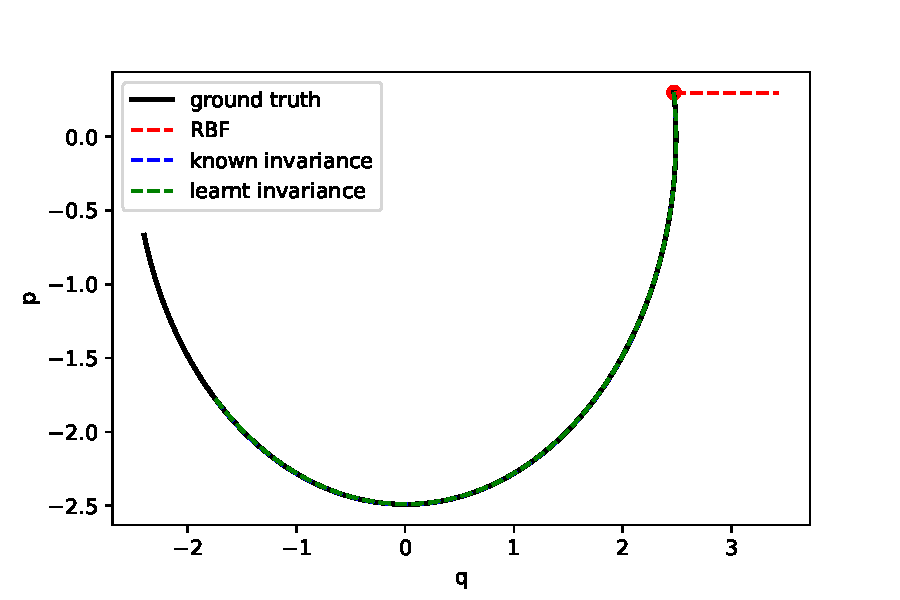
\includegraphics[width=0.8\linewidth]{../codes/figures/shm_predicted.pdf}
        \caption{One SHM predicted trajectory. We can see the baseline RBF kernel is completely unable to predict. On the other hand, the invariance constraints greatly improve the generalisability of the model and give precise prediction.}
        \label{fig:shm_prediction}
\end{figure}

\begin{figure}[H] 
  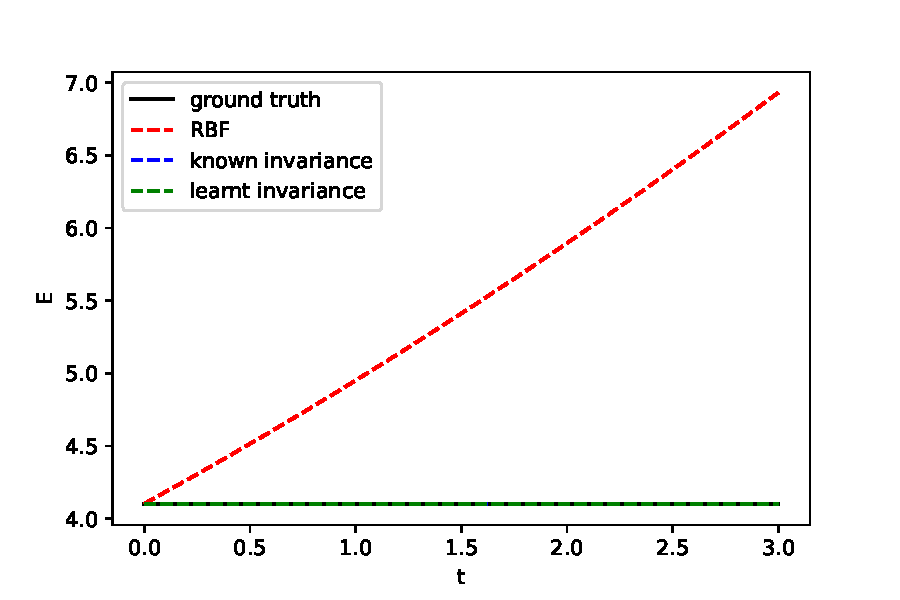
\includegraphics[width=0.8\linewidth]{../codes/figures/shm_energy.pdf}
  \centering
  \caption{The energy along the trajectory. We can again see the energy of RBF is not conserving at all as expected due to poor performance in prediction while the invariance kernel are preserving the energy perfectly.}
  \label{fig:shm_energy}
\end{figure}

\begin{figure}[H] 
  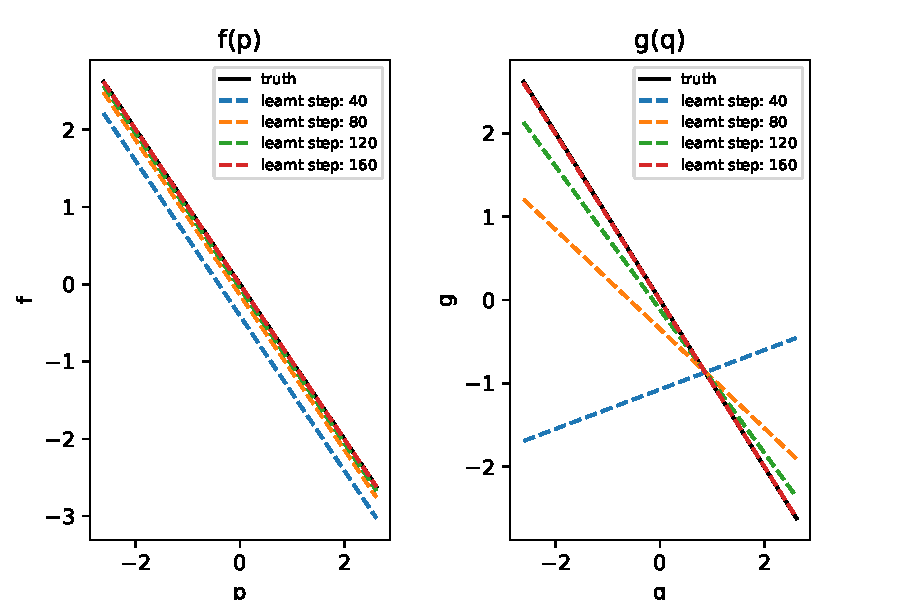
\includegraphics[width=0.8\linewidth]{../codes/figures/shm_learnt_over_time.pdf}
  \centering
  \caption{Learnt invariance for SHM. We can see the polynomials converge to the correct invariance as the algorithm trains, which are both linear in this case with $f(p)=p$ and $g(q)=q$.}
  \label{fig:shm_learnt}
\end{figure}

\begin{figure}[H]
     \centering
     \begin{subfigure}[b]{\linewidth}
        \centering
        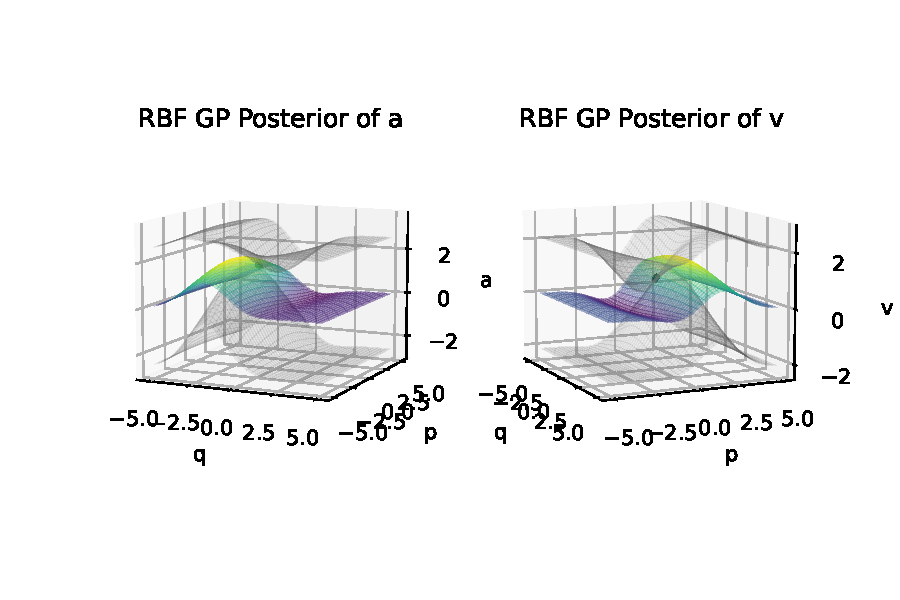
\includegraphics[width=\linewidth]{../codes/figures/posterior_shm_rbf.pdf}
        \caption{SHM RBF posterior}
        \label{fig:posterior_shm_rbf}
     \end{subfigure}
     \hfill
     \begin{subfigure}[b]{\linewidth}
         \centering
         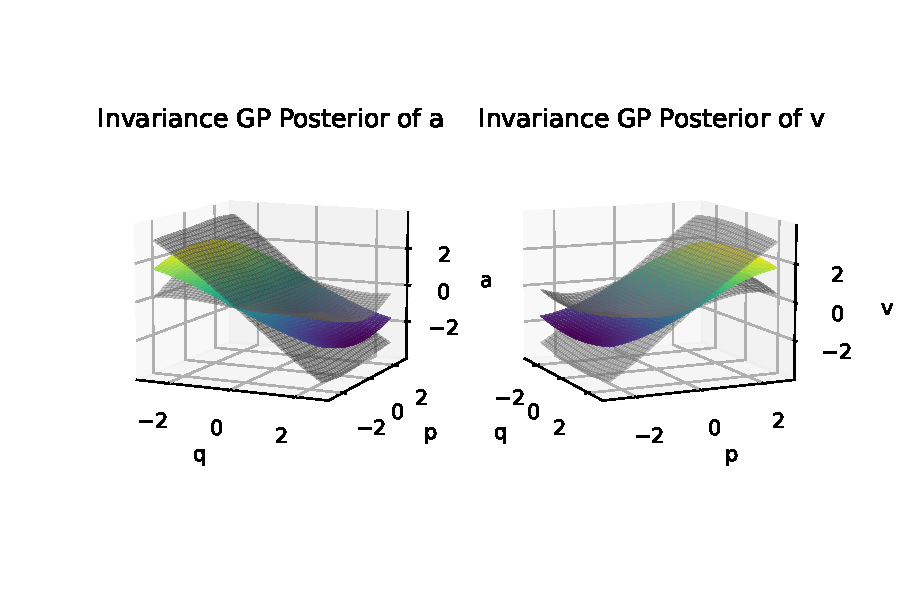
\includegraphics[width=\linewidth]{../codes/figures/posterior_shm_invariance.pdf}
         \caption{SHM invariance posterior}
         \label{fig:posterior_shm_invariance}
     \end{subfigure}
        \caption{SHM posteriors. We see here the two posteriors have different fit, which leads to different predictive power. Here the invariance kernel generalise much better due to the invariance constraints while the RBF clearly fall back to zero mean prior away from the data points (plotted as black dots).}
        \label{fig:posterior_shm}
\end{figure}

From table \ref{tab:shm_performance} as well as the sample predicted trajecetory in figure \ref{fig:shm_prediction}, we can clearly see the naive RBF kernel failed to generalise beyond the training points, and hence the poor prediction performance. 
As shown in figure \ref{fig:posterior_shm_rbf}, the GP mean falls back to zero away from the training points (the black dots), so that it is only able to predict well in the region where the data locate, which is reasonable and expected since the data is its only source of information. 
In contrast, from \ref{fig:posterior_shm_invariance} and the prediction performance, we can see the invariance kernel has much better generalisation ability and therefore the predictive power.
From the energy plot in figure \ref{fig:shm_energy}, we see both the known and learnt invariance maintain the invariance very well while the RBF kernel does not obey it at all.
In this case, the learnt invariance performs very close to the known form, as we can also see in figure \ref{fig:shm_learnt}, and has successfully recovered the physics: $f(p)=p, g(q)=q$. 
The very slight deviation is due to the fact that we cannot shrink the terms that are supposed to be zero, such as the intercept, to exactly zero, which makes the invariance slightly less accurate, and therefore the predictive performance of the learnt invariance will suffer compare to the known form.


\subsection{Nonlinear Pendulum}
The derivation of the kernel is pretty much the same for nonlinear system as the linear cases; 
however, the fitting of statistical model is expected to be more difficult since usually, nonlinear functions are more difficult to solve or learn accurately.
A simple nonlinear system in every day life is a simple pendulum as shown in figure \ref{fig:pendulum_diagram} below, where $q$ is the angle of displacement from the vertical dotted line, and $p$ is the angular velocity.

\begin{figure}[H]
        \centering
        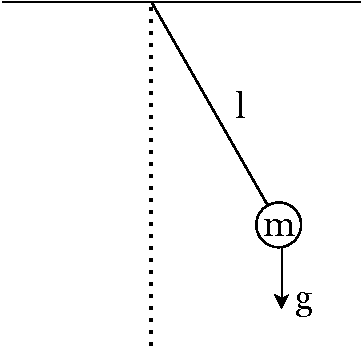
\includegraphics[width=0.3\linewidth]{../figures/pendulum.pdf}
        \caption{A pendulum is a simple system that is nonlinear, largely because the gravity $g$ acts at an angle to the displacement of the mass.}
        \label{fig:pendulum_diagram}
\end{figure}

The governing equation is 
$$
\frac{d^2q}{dt^2}=-\frac{g}{\ell}\sin q, 
$$
where $g$ is the gravitational constant that controls the gravitational force pulling down the mass of pendulum and $\ell$ is the length of the pnedulum.
We have an example trajectory in figure \ref{fig:pendulum_trajectory}, where we can see the effect of nonlinearity on the shape being not perfectly circular or ellpitical; instead, it has a roughly smooth diamond outline. 
The nonlinear dynamics arises from the sinusoidal term in the differential equations, which will complicate the derivation for invariance kernel slightly. 
Note that at small angles, $\sin x \approx x$ , so this system is approximately linear under small displacement. 
Generally, there is no analytical solution to this nonlinear problem besides the small displacement case, which will be one-dimensional SHM we saw earlier.

\begin{figure}[H] 
  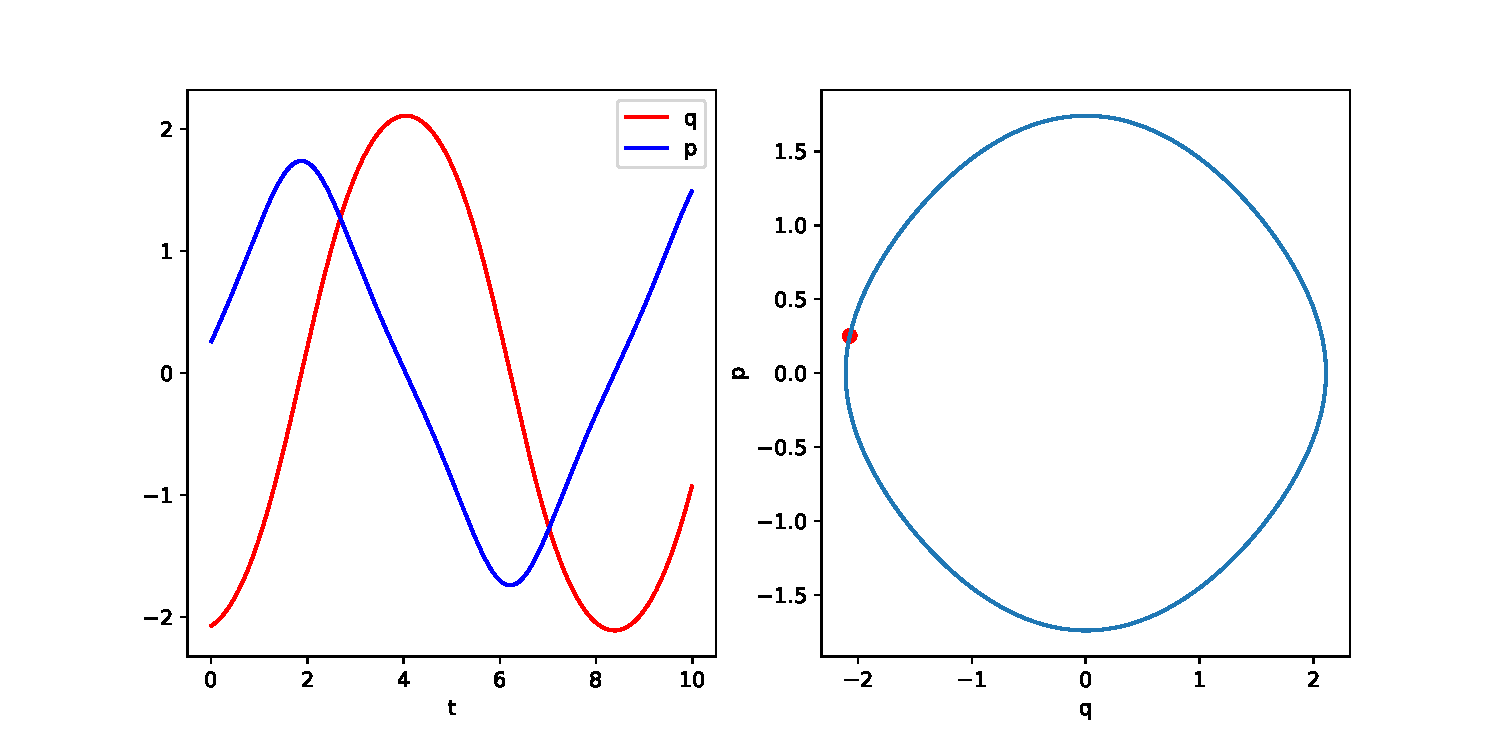
\includegraphics[width=0.7\linewidth]{../codes/figures/pendulum_trajectory_1D.pdf}
  \centering
  \caption{Example trajectory of pendulum. We can tell its nonlinearity from the nonsmooth shape of the trajectory.}
  \label{fig:pendulum_trajectory}
\end{figure}

For pendulum, we have energy $E=\frac{m\ell^2p^2}{2}+mg\ell(1-\cos q)$, and by setting its time derivative to 0, we have 
$$L[\mathbf{f}]=\frac{dE}{dt}=m\ell^2pa+mg\ell(\sin q)v=0$$
We can cancel out the common term $m\ell$ since their product cannot be zero, we have our invariance condition 
$$L[\mathbf{f}]=\ell pa+g(\sin q)v=0$$
For the derivation of our kernel, most of the terms are unchanged from the linear case in equation \ref{equ:jointABCD} and \ref{equ:ABCD}. 
However, this time, 
$$
\begin{gathered}
B=\begin{pmatrix}
    K_{RBF,a}(X, X_L) \\ K_{RBF,v}(X, X_L) \\
\end{pmatrix}\odot \begin{pmatrix}
    \ell P_L \\ g\sin(Q_L)
\end{pmatrix},\\ D=K_{RBF,a}(X_L, X_L)\odot \ell^2(p_L\otimes p_L) + K_{RBF,v}(X_L, X_L)\odot g^2(\sin(q_L)\otimes \sin(q_L)),
\end{gathered}
$$
where 
$$
\sin(Q_L) = g\begin{pmatrix}
  \sin(q_{L,1})  & \dots & \sin(q_{L,\ell})  \\
  \vdots & \text{reqeats n rows} &  \vdots\\
  \sin(q_{L,1})  & \dots & \sin(q_{L,\ell})  \\
\end{pmatrix},
$$
$$
\sin(q_L)\otimes \sin(q_L)=\begin{pmatrix}
  \sin(q_{L,1})^2 & \sin(q_{L,1})\sin(q_{L,2}) & \dots & \sin(q_{L,1})\sin(q_{L,\ell}) \\
  \vdots & \vdots & \vdots & \vdots \\
  \sin(q_{L,\ell})\sin(q_{L,1}) & \sin(q_{L,\ell})\sin(q_{L,2}) & \dots & \sin(q_{L,\ell})^2 \\
\end{pmatrix},
$$
and this is derived in the exactly same way as the linear case by computing the covariance manually. 
If we wish to parametise the invariance, it will be the same expressions as before in equation \ref{equ:joint_ABCDp} and \ref{equ:ABCDp}.
We can look at the different priors in figure \ref{fig:priors}, which showcases the baseline kernel RBF, SHM invariance kernel, as well as the pendulum invariance kernel.

We can see while the mean is zero (the assumption), the uncertainty parts reflects the form of invariance; such as the plane of SHM and the sinusoidal nature of pendulum invariance in \ref{fig:prior_pendulum_invariance} (left).

\begin{figure}[H]
     \centering
     \begin{subfigure}[b]{0.6\linewidth}
        \centering
        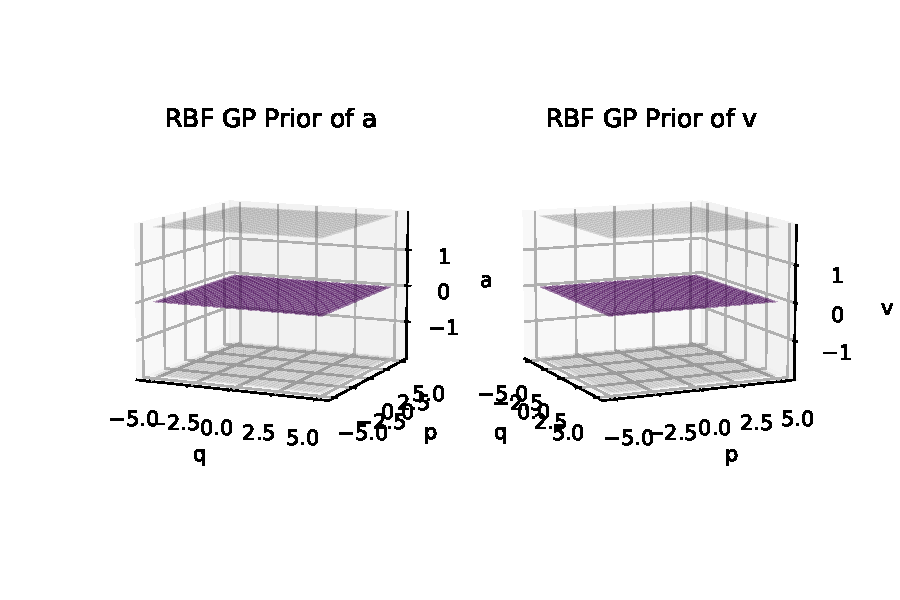
\includegraphics[width=\linewidth]{../codes/figures/prior_shm_rbf.pdf}
        \caption{RBF prior}
        \label{fig:prior_shm_rbf}
     \end{subfigure}
     \hfill
     \begin{subfigure}[b]{0.6\linewidth}
         \centering
         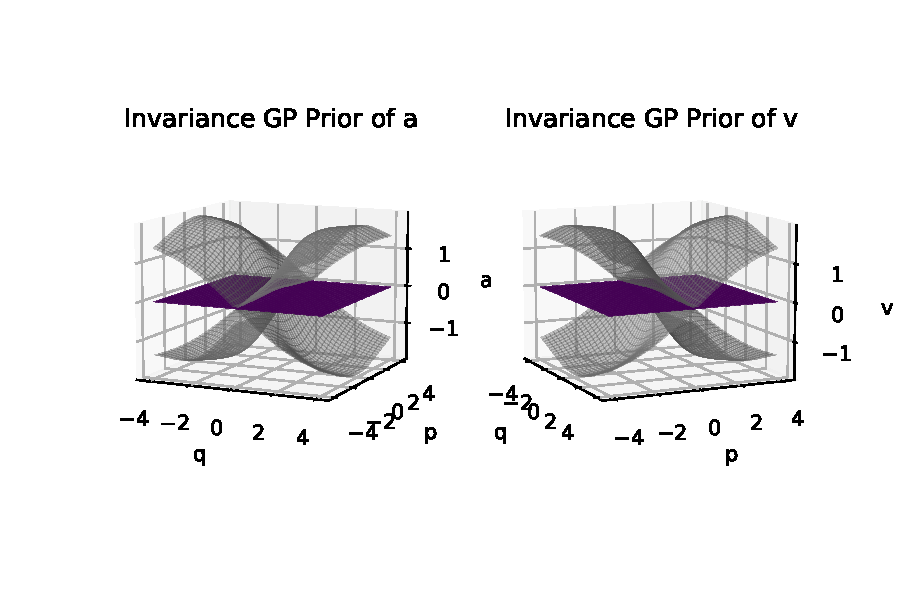
\includegraphics[width=\linewidth]{../codes/figures/prior_shm_invariance.pdf}
         \caption{SHM invariance prior}
         \label{fig:prior_shm_invariance}
     \end{subfigure}
     \hfill
     \begin{subfigure}[b]{0.6\linewidth}
         \centering
         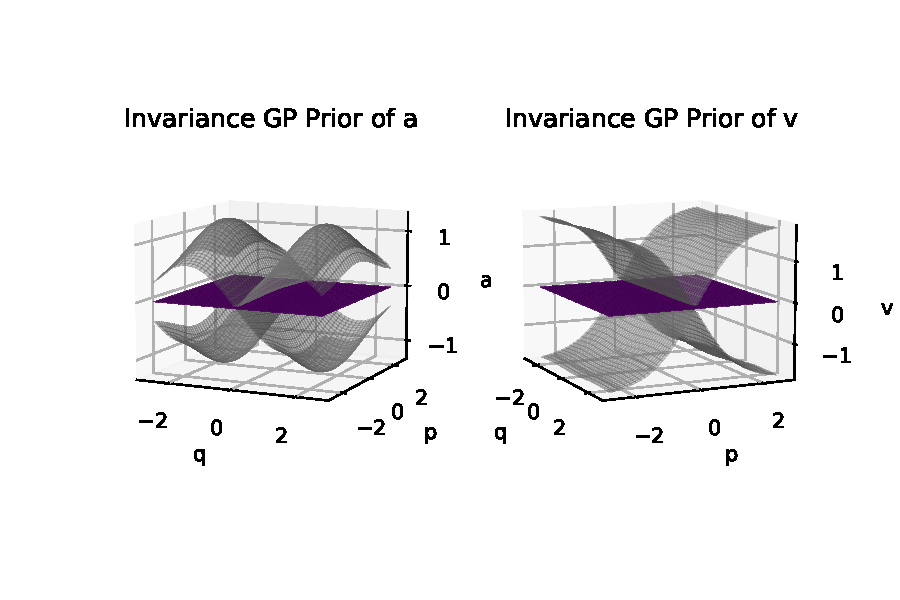
\includegraphics[width=\linewidth]{../codes/figures/prior_pendulum_invariance.pdf}
         \caption{Pendulum invariance prior}
         \label{fig:prior_pendulum_invariance}
     \end{subfigure}
        \caption{Priors of different invariance kernel. We can see the form of invariance will influence the shape of the prior, and therefore affect the model fitting, which is the inductive bias in action.}
        \label{fig:priors}
\end{figure}

For the implementation of pendulum invariance model, the experiment setup is essentially exactly the same as the SHM case. 
However, since this time the dynamics is more complicated, we will draw 3 different starting points for training between $q=\pm 150^{\circ}$ and $\pm 30^{\circ}$ for $p$, so in total 30 points.
It is also necessary since otherwise it is difficult for the polynomial to learn a nonlinear function if we only have a very small range of input.
We choose $p$ to have smaller range so the pendulum will not overshoot the $q=\pm 180^\circ$ since then the dynamics change and we would not able to use the same kernel.
We again use an invariance density of 40 between $\pm 180^{\circ}$.
We have the prediction performance of ten test trajectories summarised in table \ref{tab:pendulum_performance} as well as the sample trajectory in figures \ref{fig:pendulum_prediction} and energy along the trajectory in figure \ref{fig:pendulum_energy}.
Finally, we have the posteriors in \ref{fig:posterior_pendulum}.
The learnt polynomial is plotted in figure \ref{fig:pendulum_learnt}.

\begin{table}[H]
  \centering
  \begin{tabular}{ l l l l}
    \hline
Method           & RBF & Known Invariance&  Learnt Invariance\\
                    \hline
Log Marginal Likelihood & 299.12 & 331.66 & 325.76 \\
MSE & 0.0021 & 0.0009 & 0.0006 \\
    \hline
  \end{tabular}
  \caption{Pendulum performance. We can see again using the invariance kernel greatly outperforms the RBF. Interestingly, the learnt invariance performs slightly better than the known form. We attribute that to be due to slight overfitting of the paramters in polynomials since the input space is quite small in our case.}
  \label{tab:pendulum_performance}
\end{table}

\begin{figure}[H]
        \centering
        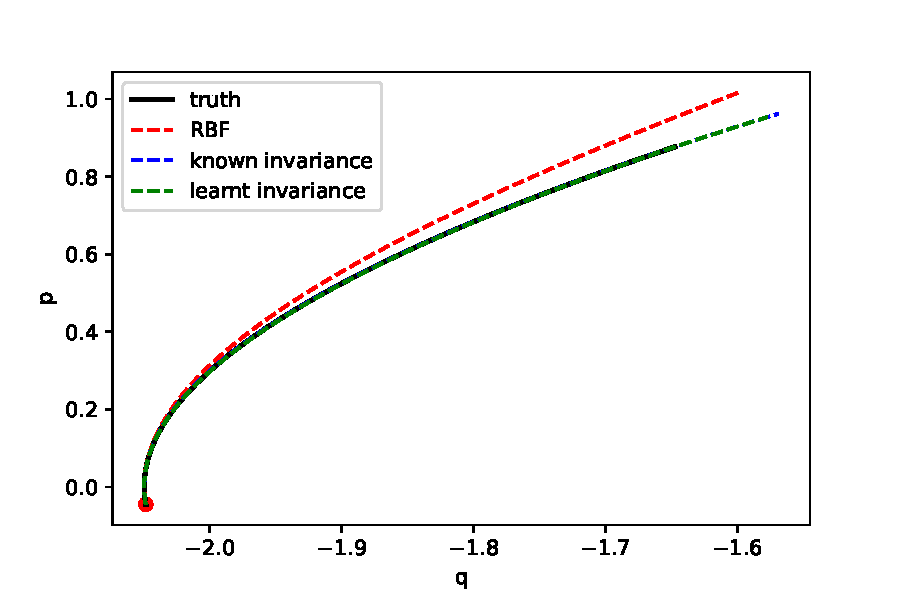
\includegraphics[width=0.8\linewidth]{../codes/figures/pendulum_predicted.pdf}
        \caption{Pendulum predicted trajectory. We see that the invariance kernel outperforms the RBF, with the known and learnt invariance overlaps. The overshoot of the trajectory is likely due to the fact that our time step is not small enough so the numerical integration will drift and slightly overshoot.}
        \label{fig:pendulum_prediction}
\end{figure}

\begin{figure}[H] 
  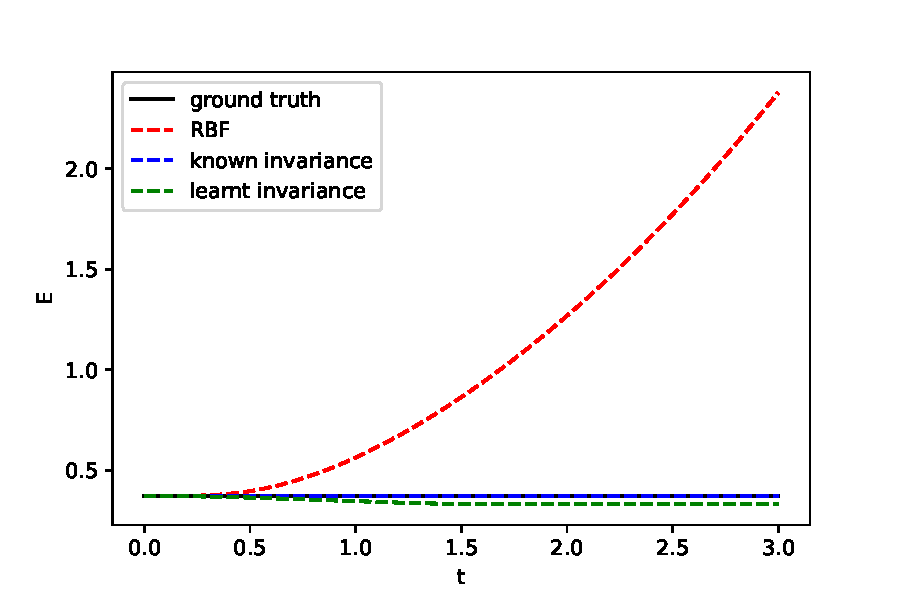
\includegraphics[width=0.8\linewidth]{../codes/figures/pendulum_energy.pdf}
  \centering
  \caption{Energy of the trajectory. We again see invariance kernels almost perfectly conserve the energy while the RBF does not have the imposed constraints.}
  \label{fig:pendulum_energy}
\end{figure}

\begin{figure}[H] 
  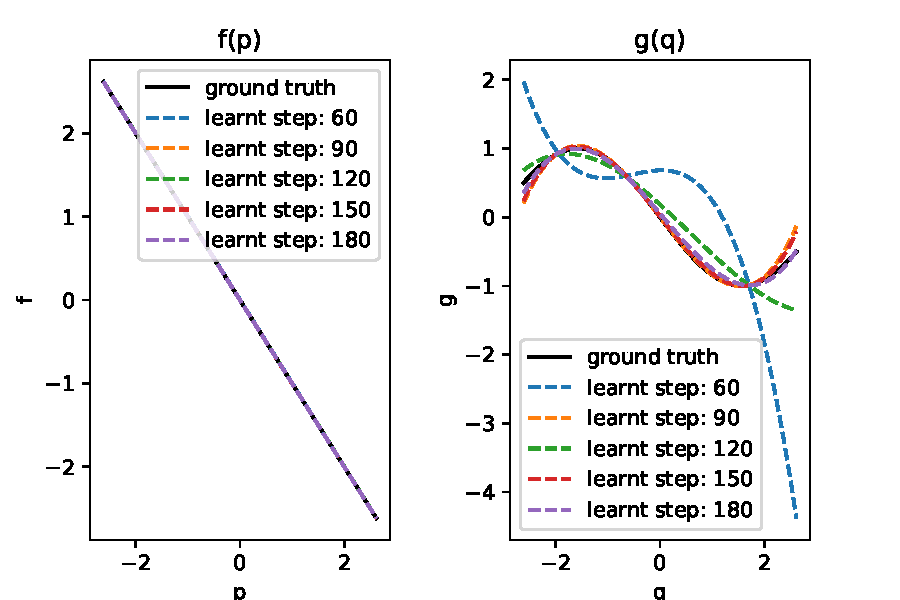
\includegraphics[width=0.8\linewidth]{../codes/figures/pendulum_learnt_over_time.pdf}
  \centering
  \caption{Learnt invariance for pendulum. We again see the polynomial converge to the true function $g(q)=\sin(q)$ and $f(p)=p$ over time.}
  \label{fig:pendulum_learnt}
\end{figure}

\begin{figure}[H]
     \centering
     \begin{subfigure}[b]{\linewidth}
        \centering
        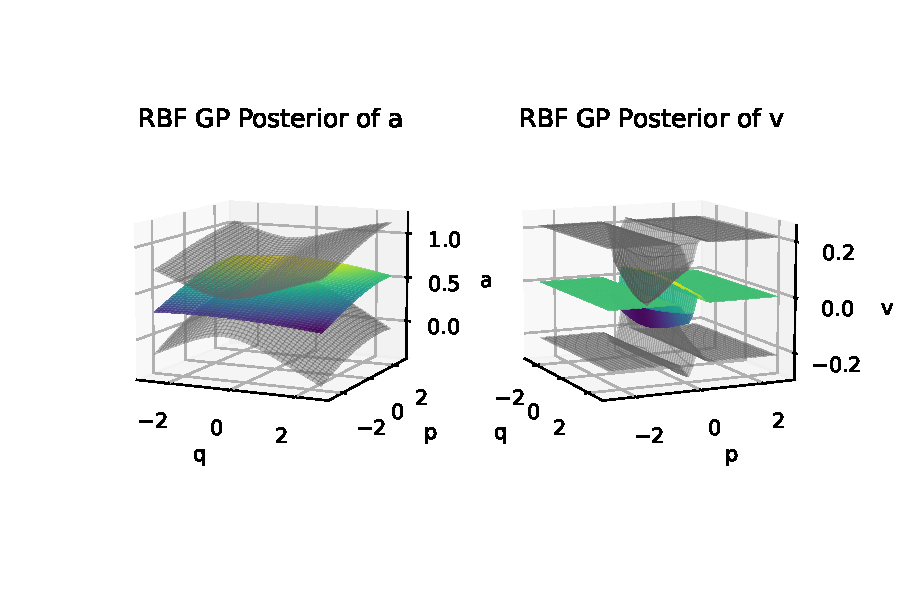
\includegraphics[width=\linewidth]{../codes/figures/posterior_pendulum_rbf.pdf}
        \caption{Pendulum RBF posterior}
        \label{fig:posterior_pendulum_rbf}
     \end{subfigure}
     \hfill
     \begin{subfigure}[b]{\linewidth}
         \centering
         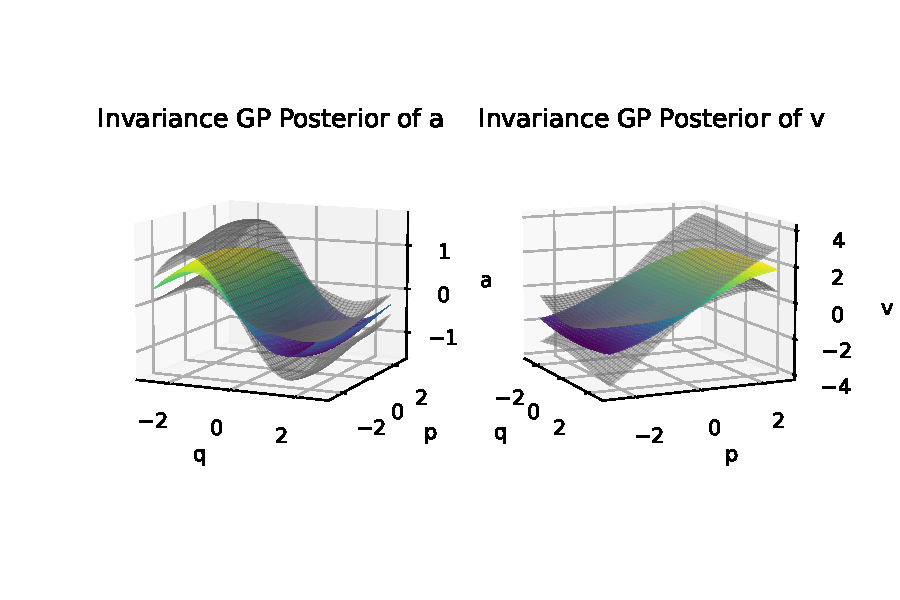
\includegraphics[width=\linewidth]{../codes/figures/posterior_pendulum_invariance.pdf}
         \caption{Pendulum invariance posterior}
         \label{fig:posterior_pendulum_invariance}
     \end{subfigure}
        \caption{Pendulum posteriors. Compare to SHM, there is less difference visually between the two posteriors for $a$. Nevertheless, the invariance still is much more accurate for $v$, which we expect it to be $v=p$, a plane.}
        \label{fig:posterior_pendulum}
\end{figure}

From table \ref{tab:pendulum_performance}, figure \ref{fig:pendulum_prediction}, we again see the RBF kernel performs poorly in generalisation and perdictive performance as well as conserving energy in figure \ref{fig:pendulum_energy}.
On the other hand, the invariance kernels predict almost exactly the ground truth again, the slight deviation (the overshoot in figure \ref{fig:pendulum_prediction}) is likely to be due to the not very small time step size (0.01) in the numerical integration. 
Surprisingly, we see the learnt invariance is slightly better in predicting, it might be due to the extra flexbility of polynomial coefficients that allow it to overfit the data a bit. 
Because our input space is relatively quite small, it is possible this overfitting leads to better predictive performance due to chances.
If we have larger input size, we would expect the learnt invariance kernel to be worse in predicting as in the SHM case.
For the energy conservation, both known and learnt invariance obeys the invariance very well from figure \ref{fig:pendulum_energy}.
Neverthless, if we zoom in to the figure, we see a very slight devivation of the learnt invariance from being completely flat, which is expected since we are approximating the $\sin(x)$ with a cubic polynomial, so this difference is expected and can be tolerated.
We can then see the learning of the polynomial in figure \ref{fig:pendulum_learnt}, the learnt polynomial is actually pretty accurate when it is optimised (of course it cannot be 100\% accurate), demonstrating that marginal likelihood is a good objective function to identify the correct invariance of a system.
From the posteriors in \ref{fig:posterior_pendulum}, we see RBF generalise much better in $a$ thanks to extra data points we feed in, but its learning in $v$ is still relatively poor compare to the invariance kernel, where it correctly identify $v=p$ a plane that is independent of $q$.

Note that although it may seem in this case, there is not as significant a difference in prediction performance between baseline and invariance kernel as the SHM case, it is because the input space is relatively small, so that RBF is able to fit better.
We need to provide more data because of the fitting of polynomial requires a wider range of data to fit the curvature of $\sin(x)$. 
In fact, if we know the invariance a priori, then we only need ten data points to fit well as shown in figure \ref{fig:data_efficiency}.
We can imagine if our input spaces is much larger, the RBF kernel will fail to generalise beyond where data locates and invariance kernel will still able to predict well once the invariance is successfully learnt since the invariance constraints are global.
This is evident from the learning of $v$ dynamics, where RBF fails to learn the plane and the invariance kernel is able to extend the constraints to a much larger distance.

We wish to compare quantitatively how good is invariance kernel compare to RBF in terms of data efficiency. 
To investigate, we sample a test trajectory and feed the RBF kernel increasingly more data points until it converges to the ground truth while we simply provide the known invariance kernel with 10 data points.
The result is shown in figure \ref{fig:data_efficiency}. 
We see that with invariance kernel, it is at least ten times more data efficient than the baseline RBF.

\begin{figure}[H] 
  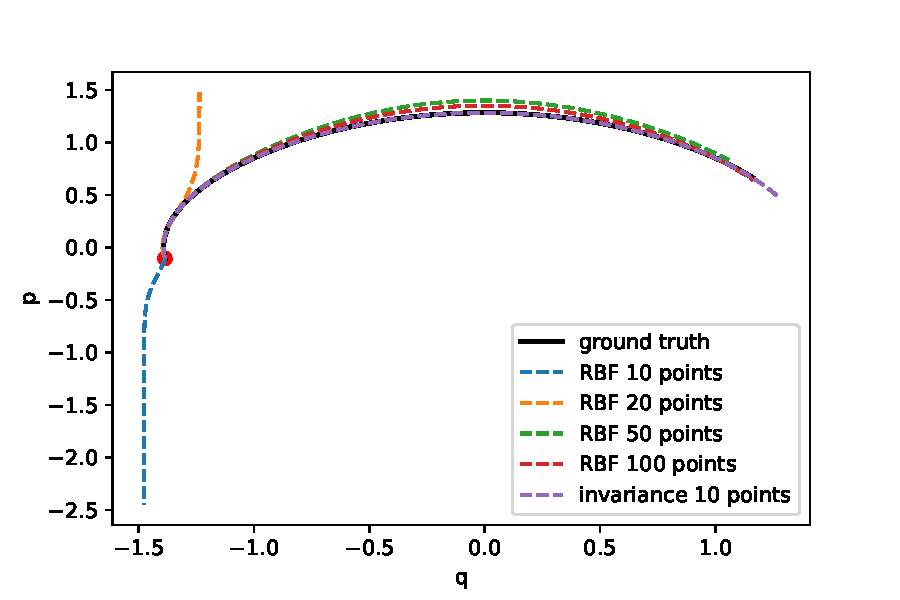
\includegraphics[width=0.8\linewidth]{../codes/figures/data_efficiency.pdf}
  \centering
  \caption{Data efficiency comparison. We see the invariance kernel needs 10 times less data points to predict accurately compare to RBF, demonstrating how data efficient it can be by embedding inductive bias.}
  \label{fig:data_efficiency}
\end{figure}

\section{Invariance Density}
The number of invariance points may seem to be arbitrarily chosen. 
How many of these invariance points do we actually need to achieve a good result and can there be too many invariance points such that the GP has too many constraints and too little degree of freedom?
Would this causes the GP to remain zero, where the invariance is trivally satisfied (everything is zero) because it is too contraint?
Here we will to explore how different invariance density affect the performance of the kernel as well as the degree of freedom.
The effective degrees of freedom is calculated by the trace of $K(K+\sigma^2_n\mathbb{I}^{-1})$ (\cite{rasmussen_williams_2006}), where $K$ is the kernel.
Since one-dimensional SHM is trival to learn, we test it on the nonlinear pendulum case.
We will use different invariance density using the same training data and a random test trajectory.
We again calculate the MSE of trajectory prediction as well as the percentage of energy deviation from the starting point from the start to end of a trajectory.
The results is shown in figure \ref{fig:vary_invariance_density}.

\begin{figure}[H] 
  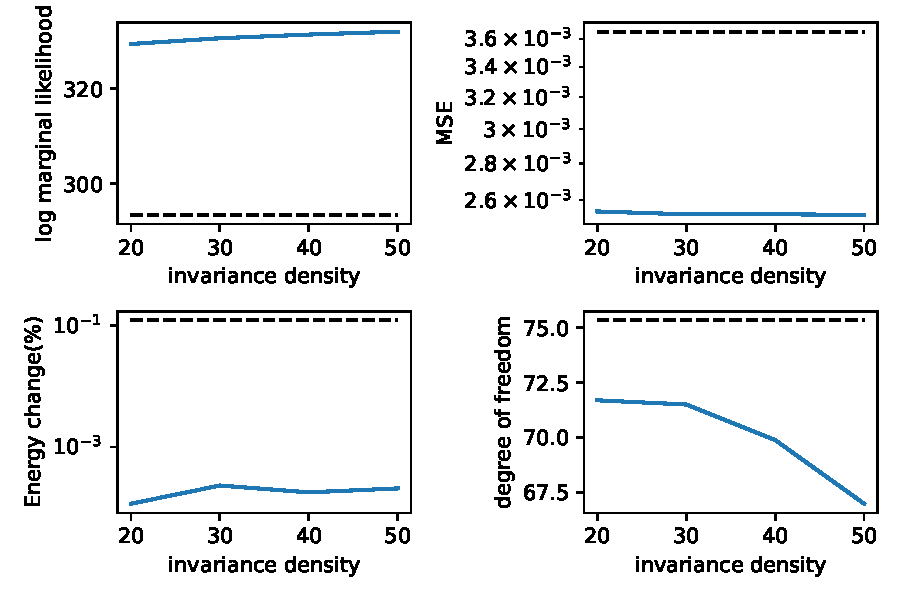
\includegraphics[width=0.8\linewidth]{../codes/figures/vary_invariance.pdf}
  \centering
  \caption{Effect of varying invariance density on performance of GP.}
  \label{fig:vary_invariance_density}
\end{figure}

We have the black dotted line serving as the baseline (RBF).
We can see that for the marginal likelihood, it increases as the number of invariance points increases, which is expected since we have more information/evidence to support the data.
However, there is not that large a difference and it seems to have diminishing return.
Same thing happened with MSE, where it essentially remains the same.
A similar observation is made with conservation of energy, where the invariance density almost has no effect. 
Lastly, we see the degree of freedom decrease as we increase the invariance density, which is expected again since more constraints should lead to fewer degrees of freedom.
Importantly, we see there is actually that much decrease in degree of freedom compare to the RBF, which assures us that our invariance model is not too restrictive and also answers the question in section 3.3, where we wonder to what extent is the problem solved by using the invariance kernel.
The answer is essentially not that much as there is still plenty of degrees of freedom.

Overall, we see there is not that big an advantage to increase our invariance density beyond a certain point due to diminishing return in performance and $N^6$ computational cost, where $N$ is the invariance density ($M^3$ in inverting matrix of size $M\times M$ and total $M=N^2$ points).
Therefore, from this point we will choose the smallest invariance density that give reasonable performance.  


\section{Damped System}
Now we move on to the damped version of the previous two systems. 
We will then used the methods, approximate invariance and latent dyanmics, described in section 3.2 and section 3.4 along with the invariance kernels derived in section 4.4.1 and section 4.4.2, to modify our GP model. 
For the data, we will model the system as a damped SHM or pendulum with linear velocity dependent force.
If we denote $\omega_0^2=k/m$ or $\omega_0^2=g/\ell$
we will have the equation of motion for SHM and pendulum respectively as
$$
\frac{d^2q}{dt^2}+2\gamma\frac{dq}{dt}+\omega_0^2q=0;\ \frac{d^2q}{dt^2}+2\gamma\frac{dq}{dt}+\omega_0^2\sin q=0 ,
$$
and the $\gamma$ is the damping factor that controls how strong the frictional force is, with $q$ having the same meaning as before. 
Note that we will only focus on underdamping case ($\gamma < \omega_0^2$) so that the system still oscillate but with gradually reduced amplitude instead of critical damped ($\gamma=\omega_0^2$) or overdamped ($\gamma>\omega_0^2$) case where the system simply slowly decays to still.
An example trajectory for damped SHM and damped pendulum is shown below in figure \ref{fig:damped_trajectory}.
For the damping, we will choose $\gamma= 0.1$, which is fairly damped as shown in figure \ref{fig:damped_pendulum_trajectory}, \ref{fig:damped_shm_trajectory}, where we see the amplitude slowly decreases as the trajectory spirals in. 

\begin{figure}[H]
     \centering
     \begin{subfigure}[b]{\linewidth}
        \centering
        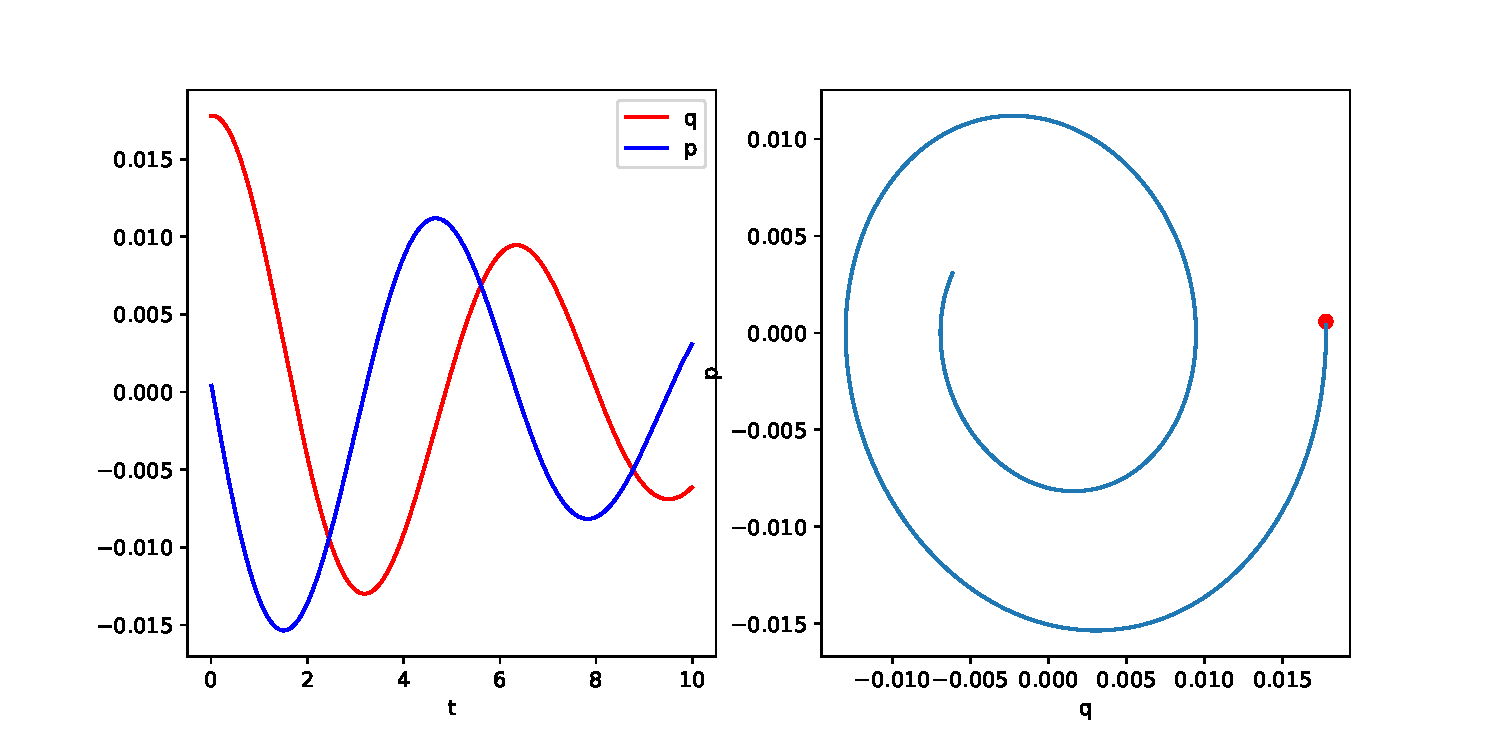
\includegraphics[width=0.5\linewidth]{../codes/figures/damped_shm_trajectory_1D.pdf}
        \caption{Example trajectory of damped SHM}
        \label{fig:damped_shm_trajectory}
     \end{subfigure}
     \hfill
     \begin{subfigure}[b]{\linewidth}
        \centering
        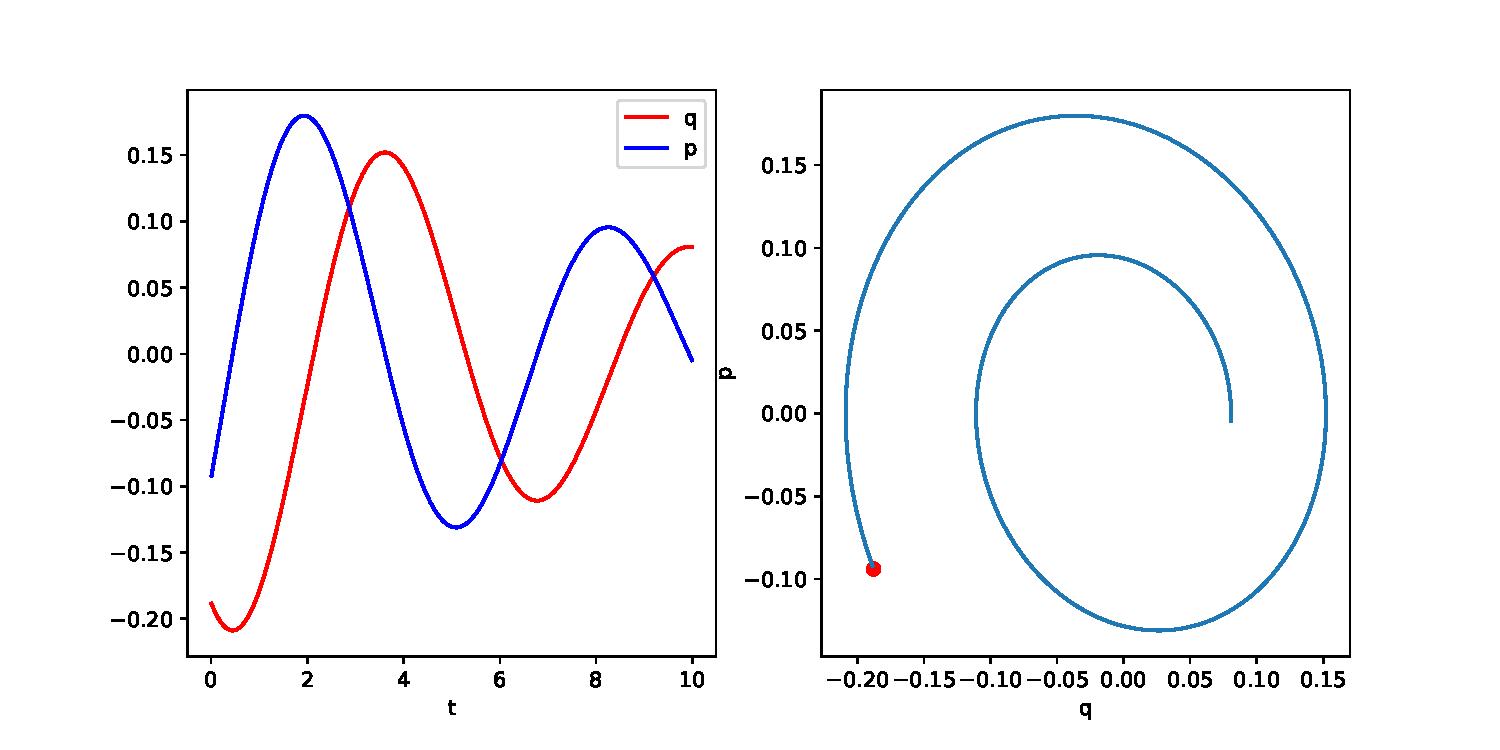
\includegraphics[width=0.5\linewidth]{../codes/figures/damped_pendulum_trajectory_1D.pdf}
        \caption{Example trajectory of damped pendulum}
        \label{fig:damped_pendulum_trajectory}
     \end{subfigure}
        \caption{Example trajectories of damped systems, with damping factor $\gamma=0.1$. We can tell it is damped by its sprialed in trajectory.}
        \label{fig:damped_trajectory}
\end{figure}

As mentioned in section 3.4, we can invent a latent variable, $z$, to account for the dissiaptive dynamics.
We can integrate out the $z$ to get the marginal distribution of the observed dynamics; at the same time, we can also condition the latent variable on the observed dynamics to obtain the posterior distribution of this latent disspative dynamics.
In our cases of damped pendulum and SHM, we can actually derive the expression of this latent disspative dynamics. 
Note that however, this requires physics knowledge, $p=v$, where we previously assumed to not known a priori.
As a result, in general dynamical systems we would not be able to derive the analytical form of $z$ as a function of $p, q$ (we could still obtain its posterior, but we cannot verify its correctness).

If we have damped SHM, we knew that $E=\frac{mp^2}{2}+\frac{kq^2}{2}$, then as before $\frac{dE}{dt}=mpa+kqv$.
Using our knowledge of $p=v=\frac{dq}{dt}$, we have $\frac{dE}{dt}=mva+kvq=v(ma+kq)$.
From the differential equation $\frac{d^2q}{dt^2}+2\gamma \frac{dq}{dt} +\frac{kq}{m}=0$, we can write it as $m\frac{dp}{dt}+2m\gamma v + kq=0$ so that $ma+2m\gamma v+kq=0$ or $ma+kq=-2m\gamma v$.
Finally, we obtain
$$
\frac{dE}{dt} = v(-bv) = -bv^2
$$
As a result, from equation \ref{equ:LEplusZ}, we identify $z=-bv^2=-bp^2$, and therefore we would expect its posterior to be quadratic in $p$ and constant in $q$.
Simliar result can be derived for damped pendulum, where we again expect $z$ to be quadratic in $p$ and independent of $q$.

\subsection{Damped SHM}
We will demonstrate here how to modify previously derived invariance kernel to accomdate the damping.
In the first case, we have approximate invariance.
We will modify equation \ref{equ:shm_invariance} according to the equation \ref{equ:damped_invariance}.
Therefore, we will have
$$
\mathbf{f}(X)|L[\mathbf{f}(X_L)]=0\sim\mathcal{N}(-B(D+\sigma^2_L\mathbb{I})^{-1}\mathbf{m}_\ell,A-B(D+\sigma^2_L\mathbf{I})^{-1}C),
$$
and as before $\sigma_L^2$ and $\mathbf{m}_\ell$ are learnable.
$A, B, C, D$ are defined as before in \ref{equ:ABCD}.

For our second method of introducing a latent dynamics, we will modify equation \ref{equ:jointABCD} according to equation \ref{equ:joint_withZ}.
By applying equation \ref{equ:LEplusZ} to SHM, we have $$L_\gamma[\mathbf{f},z]=mpa+kqv+z=0,$$ and we obtain 
$$
\begin{pmatrix}
  \begin{pmatrix}
    \mathbf{f}(X)\\z(X)
  \end{pmatrix}\\L_\gamma[\mathbf{f}(X_L), z(X_L)]
\end{pmatrix}
\sim\mathcal{N}
\left(\begin{pmatrix}
  \mathbf{0}_{3n}\\\mathbf{0}_\ell
\end{pmatrix},\begin{pmatrix}
  A & B\\ C&D\\
\end{pmatrix}\right),
$$
where now $A=K(X,X)$ with $K=\begin{pmatrix}
  K_f & 0 \\ 0 & K_z\\
\end{pmatrix}$ as in section 3.4 and $C=B^T$.
In a similar fashion to the undamped SHM invariance kernel derivation in section 4.4.1, using the form of $L_\gamma$ above we have 
$$
\begin{gathered}
B=\begin{pmatrix}
  K_{RBF,a}(X, X_L) \\ K_{RBF, v}(X, X_L) \\ K_{RBF, z}(X, X_L)\\
\end{pmatrix}
\odot \begin{pmatrix}
  mP_L \\ kQ_L \\ 1
\end{pmatrix},\\ 
D = K_{RBF, a}(X_L, X_L)\odot m^2(p_L\otimes p_L) + K_{RBF, v}(X_L, X_L)\odot k^2(q_L\otimes q_L) + K_{RBF, z}(X_L, X_L).
\end{gathered}
$$

Finally, we use equation \ref{equ:normal_condtion} and marginalisation to arrive at
$$
\mathbf{f}(X)|L_\gamma[\mathbf{f}(X_L),z(X_L)]=0 \sim \mathcal{N}(\mathbf{0}_{2n}, [A-BD^{-1}C]_{[0:2nd, 0:2nd]})
$$
as explained in section 3.4 to get our modified invariance kernel.
For the derivation of posterior of $z$, please see section 3.4 to obtain appropriate sub matrixes from $A-BD^{-1}C$.
The version for paramerterised invariance is omited since it is largely similar to what we have seen.

For experiment, we have the same setup as the original undamped SHM, with the same input range.
However, to learn the damping effect we will make the training trajectory longer to 20 time steps.
Also, we will have three random starting trajectories instead, so we have a total of 60 training points.
This is because of the damped system is harder to train, and also that we have a very flexible latent variable and we need more data points to help constrain it or else the invariance condition would be very trivally satisfied.
The results of ten test trajectories is summarised in table \ref{tab:damped_shm_performance} and with trajectory prediction in figure \ref{fig:damped_shm_prediction} and energy prediction in figure \ref{fig:damped_shm_energy}.
The learnt $f(p)$ and $g(q)$ is shown in figure \ref{fig:damped_shm_learnt}.

\begin{table}[H]
    \centering
\begin{tabularx}{\linewidth}{c|LLLLL} 
    \hline
Method           & RBF & Known Approximate Invariance&  Learnt Approximate Invariance & Known Invariance (latent) & Learnt Invariance (latent)\\
  \hline
Log Marginal Likelihood & 636 & 647 & 646 & 649 & 653 \\
MSE & 0.00142 & 0.00130 & 0.00134 & 0.00091 & 0.00101 \\
    \hline
\end{tabularx}
\caption{Damped SHM performance. We can see the approximate invariance is no longer significantly better than RBF, while the latent invariance model is much better.}
\label{tab:damped_shm_performance}
    \end{table}

\begin{figure}[H]
        \centering
        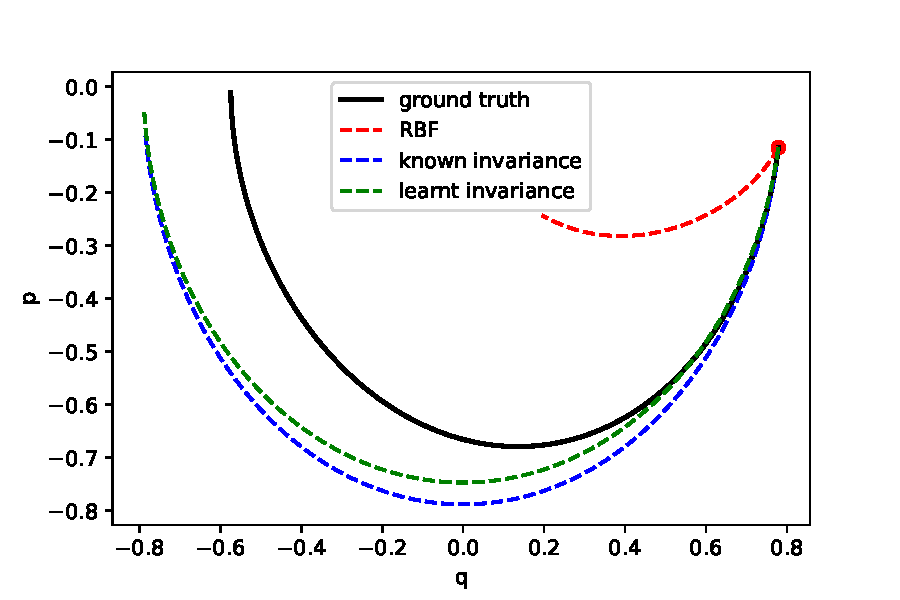
\includegraphics[width=0.8\linewidth]{../codes/figures/damped_shm_predicted.pdf}
        \caption{Damped SHM predicted trajectory. We can see the approximate invariance can no longer predict the trajectory perfectly, while the latent model is much closer to the truth.}
        \label{fig:damped_shm_prediction}
\end{figure}

\begin{figure}[H] 
  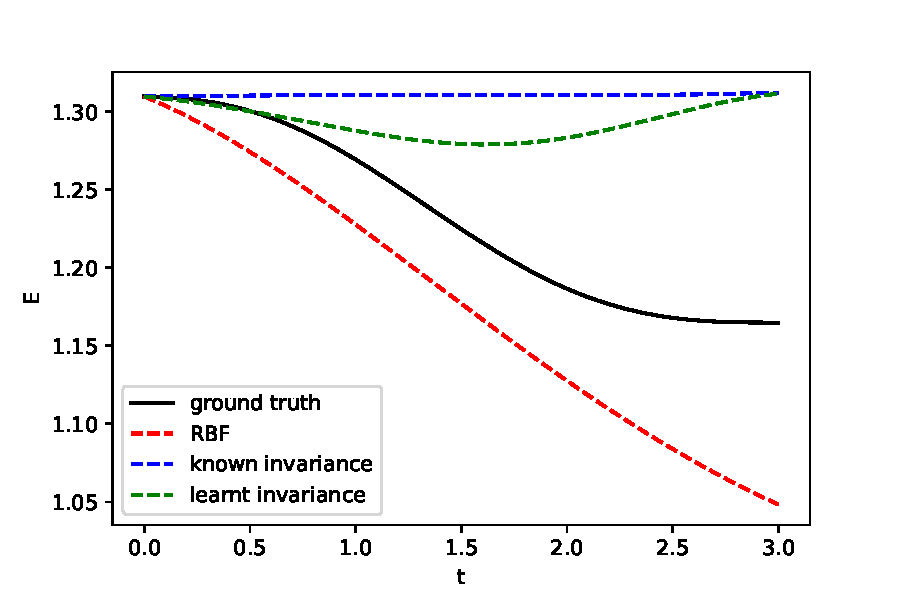
\includegraphics[width=0.8\linewidth]{../codes/figures/damped_shm_energy.pdf}
  \centering
  \caption{Energy conservation for damped SHM. We see the invariance models no longer conserve energy, and is able to dissipate energy.}
  \label{fig:damped_shm_energy}
\end{figure}


\begin{figure}[H] 
  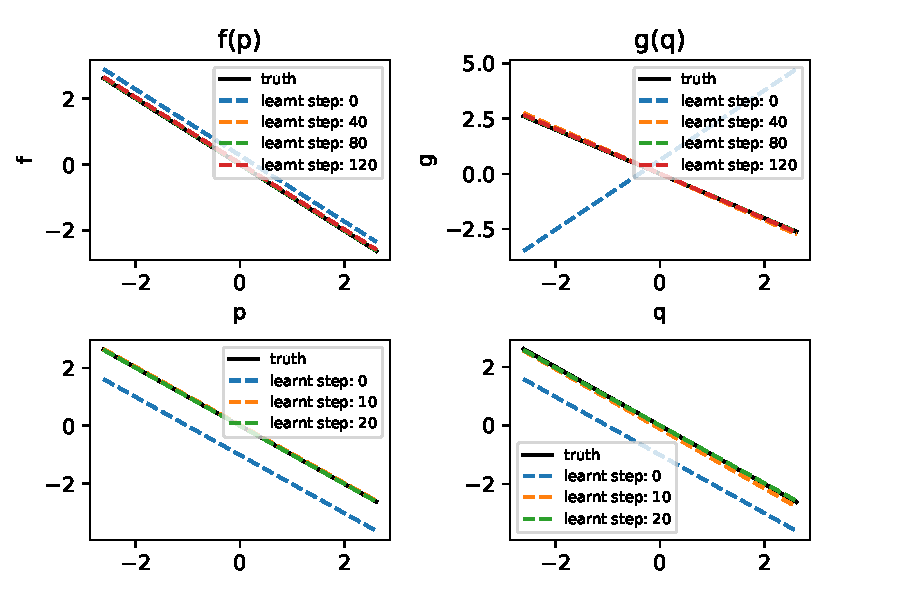
\includegraphics[width=0.8\linewidth]{../codes/figures/damped_shm_learnt_over_time.pdf}
  \centering
  \caption{Learnt invariance for damped SHM. Top: Approximate Invariance, Bottom: Latent Invariance. We see again the model is able to deduce the correct invariance even when there is damping.}
  \label{fig:damped_shm_learnt}
\end{figure}

\begin{figure}[H] 
  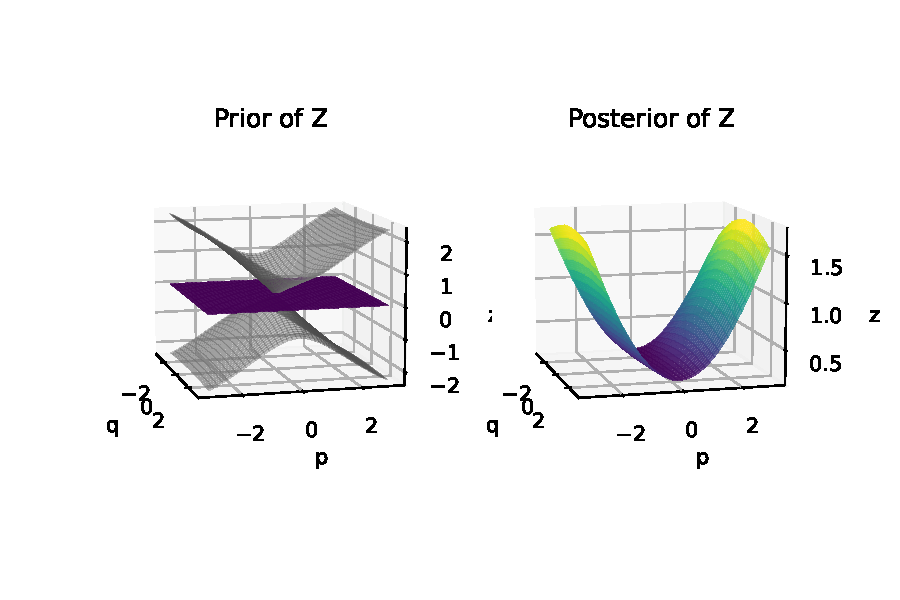
\includegraphics[width=0.8\linewidth]{../codes/figures/latent_damped_shm.pdf}
  \centering
  \caption{Latent variable distribution. We can clearly see the posterior of $z$ follows the quadratic function of $p$ while being constant in $q$ as we expected.}
  \label{fig:latent_damped_shm}
\end{figure}

From both the predicted trajectory in figure \ref{fig:damped_pendulum_prediction} and table \ref{tab:damped_shm_performance}, we can see the latent invariance kernel is much better than the approximate invariance model, which actually has similar performance (still better) than the RBF. 
The possible reasons are two folds.
Firstly, the latent model has arguably more knowledge built in than the approximate invariance. Reason being that we are explicitly using the variable to model the deviation and that varaible happens to have an exact solution in our case.
Therefore, we can expect the model to do well if the latent model is inferenced correctly.
On the other hand, the approximate invariance, being a random variable has an uncertainty that could be of wide range of values so it is difficult for it to apply the invariance knowledge for all cases.
Secondly, in a similar argument as before, we need to feed in more data to learn the damping (and invariance function).
However, at least in the case of latent disspative force, this damping is has longer range of effect since the invariance constraint is global so that once we learnt it, we can in principle apply it into a much larger input space.
As a result, we can expect there will be much bigger difference in performance between the baseline and the two invariance model in a larger input space or a more complex problem.
Bottomline, the invariance kernel still improves on the predictive performance so that the model still can take advantage of the knowledge of invariance even though it is not strictly enforced. 

For energy consevation in figure \ref{fig:damped_pendulum_energy}, we can see the latent invariance is able to learn the decrease in energy, although not very accurately.
This is possibly due to the fact that the latent disspative dynamics has to be inferred exactly to match the $\frac{dE}{dt}$ perfectly, and we have not supplied it enough data to do so.
We can see the approximate invariance almost does as badly as the RBF in fitting the correct $\frac{dE}{dt}$, which is likely because of the difficulty of finding the perfect balance between enforcing invariance while being relaxed with the constraints.
Overall, we conclude that the latent disspative dynamics model work better than the approximate invariance, which is still better than no invariance at all.

In figure \ref{fig:damped_pendulum_learnt}, we looked at whether the model is able to infer the correct invariance even when it cannot make full use of the invariance constraints.
As we can see, they still learn the correct polynomial almost perfectly, demonstrating that marginal likelihood is a robust objective to learn invariance even with disspative effect presence.
Lastly, we look at figure \ref{fig:latent_damped_shm}, where we obtain the posterior of $z$ given observed dynamics $a, v$ as well as the invariance $L_\gamma$.
It captures the true solution very well, with a well defined quadratic as a function of $p$ and no variation in the direction of $q$ (i.e. independent of $q$), which is what we expected as explained at the start of section 4.6, which is reassuring of our approach.


\subsection{Damped Pendulum}
We omit the derivation of the appropriate invariance kernel and latent dyanmics model since it is largely similar to the damped SHM case, and we simply have to swap $q$ with $\sin(q)$ at appropriate places. 
For the experiment, the setting of damped pendulum is the again the same as the undamped pendulum, with same input space.
For the input data, this time we have five different starting points since we expect the $\sin(q)$ function to be harder to learn in damped cases; but since we have more starting points, we kept the length of each trajectory to be 10 time steps, so 50 points in total.
The results is summarised in table \ref{tab:damped_pendulum_performance} and with predictions of trajectory figure \ref{fig:damped_pendulum_prediction} and energy in figure \ref{fig:damped_pendulum_energy}.
The learnt polynomial is plotted in \ref{fig:damped_pendulum_learnt}.

\begin{table}[H]
    \centering
\begin{tabularx}{\linewidth}{c|LLLLL} 
    \hline
Method           & RBF & Known Approximate Invariance&  Learnt Approximate Invariance & Known Invariance (latent) & Learnt Invariance (latent)\\
  \hline
Log Marginal Likelihood & 516 & 525 & 525 & 548 & 522 \\
MSE & 0.0012 & 0.0008 & 0.0008 & 0.0008 & 0.0008 \\
    \hline
\end{tabularx}
\caption{Damped Pendulum performance. Here the invarinace models still perform better than the RBF but this time the two methods perfrom roughly the same in predictive power.}
\label{tab:damped_pendulum_performance}
    \end{table}

\begin{figure}[H]
        \centering
        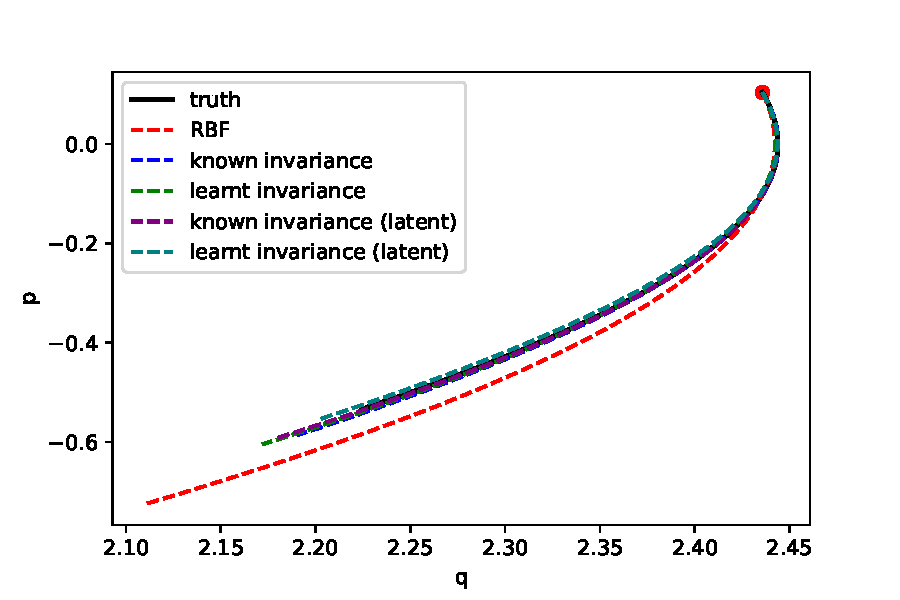
\includegraphics[width=0.8\linewidth]{../codes/figures/damped_pendulum_predicted.pdf}
        \caption{Damped pendulum predicted trajectory. Here we see the all invariance models perform similarly and better than the RBF baseline.}
        \label{fig:damped_pendulum_prediction}
\end{figure}

\begin{figure}[H] 
  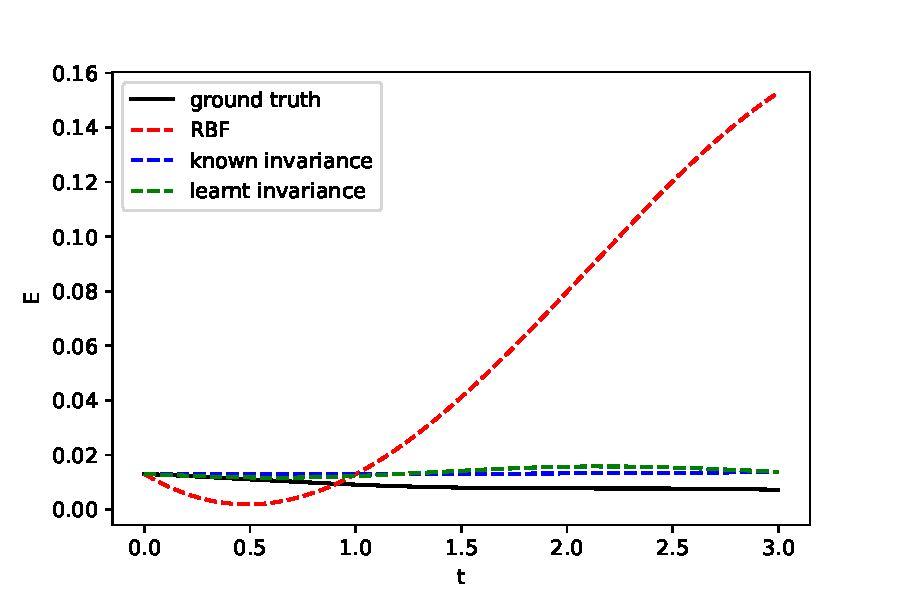
\includegraphics[width=0.8\linewidth]{../codes/figures/damped_pendulum_energy.pdf}
  \centering
  \caption{Energy conservation for damped pendulum. Again, we see that the invariance models no longer conserve energy and is able to learn the dissipation.}
  \label{fig:damped_pendulum_energy}
\end{figure}


\begin{figure}[H] 
  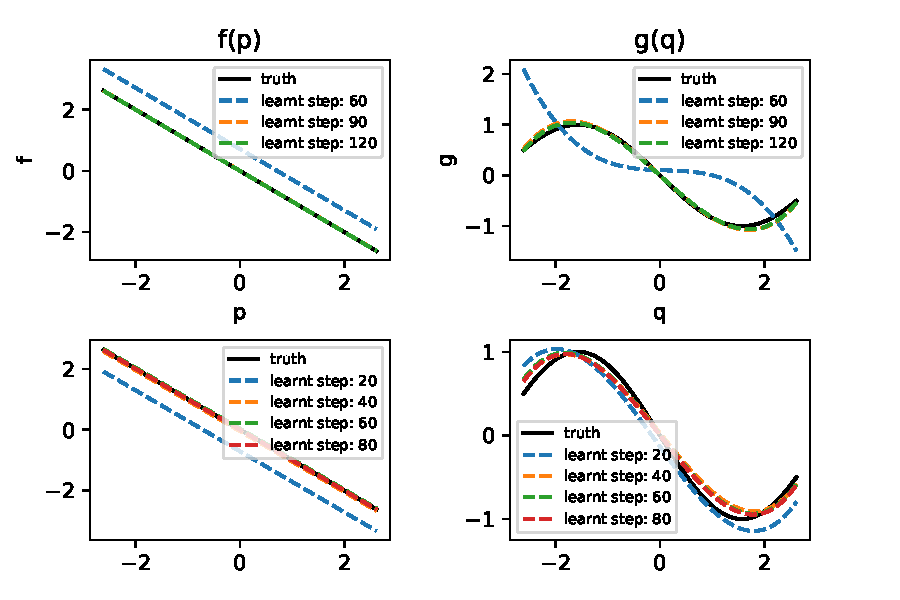
\includegraphics[width=0.8\linewidth]{../codes/figures/damped_pendulum_learnt_over_time.pdf}
  \centering
  \caption{Learnt invariance for damped pendulum. Top: Approximate Invariance, Bottom: Latent Invariance. We see the learning of invariance is fairly accurate but slightly worse in fit than the undamped case.}
  \label{fig:damped_pendulum_learnt}
\end{figure}

\begin{figure}[H] 
  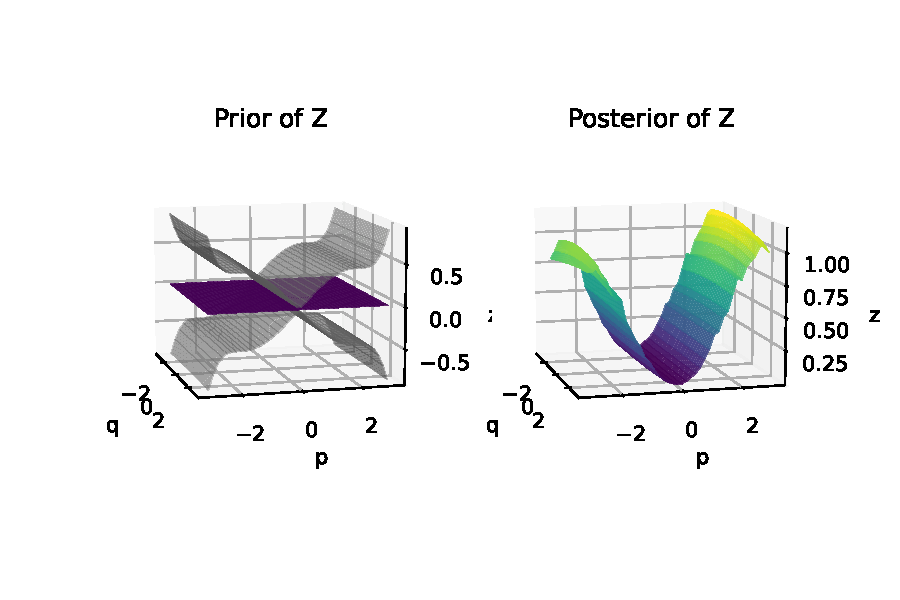
\includegraphics[width=0.8\linewidth]{../codes/figures/latent_damped_pendulum.pdf}
  \centering
  \caption{Latent variable distribution. Again, we see the quadratic behaviour as expected.}
  \label{fig:latent_damped_pendulum}
\end{figure}

From table \ref{tab:damped_pendulum_performance} and trajectory prediction in figure \ref{fig:damped_pendulum_prediction}, we can see the invariance kernel perform similarly regardless of whether it is approximate or uses latent dynamics, and are all much better in predictive performance than RBF.
The reason why this time the two approaches to invariance perform similarly is likely due to the fact that more starting points are trained than the damped SHM case (5 v.s. 3), and also that the input space is smaller so that the approximate invariance is able to capture the right amount of deviation the invariance from zero can be tolerated.
This demonstrates that the latent disspative dynamics model is still more data efficient than the approximate invariance.
Since it is a more complex nonlinear problem, the knowledge of invariance clearly is very help compare to the baseline RBF.
Again, both invariance models are able to learn almost correctly the true $\frac{dE}{dt}$ as shown in figure \ref{fig:damped_pendulum_energy}, while the RBF even increases the energy.

From figure \ref{fig:damped_pendulum_learnt}, we again see that even in the nonlinear damped system, the model is still able to learn the correct invariance, which is quite remarkable the power of using marginal likelihood to learn invarinace. 
Finally, we see the posterior of $z$ in figure \ref{fig:latent_damped_pendulum}, which is roughly quadratic in $p$ once again. 
However, it is a little bit jiggly, possibly due to the nonlinearity so it is a little bit more noisy.


\section{Two-dimensional System}
A two-dimensional system is not that different from an one-dimensional system. The major difference being there will be two more input variables and hence two more dynamics term as well. 
We will again look at two simple examples, a linear two-dimensional SHM, and a nonlinear double pendulum.

\subsection{Linear SHM}
A simple extension to one-dimensional SHM to two-dimensional is just allowing the spring to be at an angle so that the system is now in a two-dimensional space as shown in figure \ref{fig:shm_2d_diagram}, and the system is still constrained in the plane.

\begin{figure}[H]
        \centering
        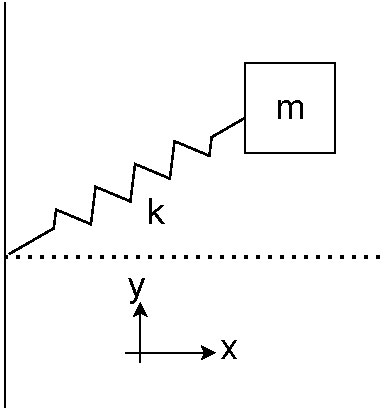
\includegraphics[width=0.4\linewidth]{../figures/2dshm.pdf}
        \caption{Two-dimensional mass-spring system exhibiting two-dimensional simple harmonic motion.}
        \label{fig:shm_2d_diagram}
\end{figure}

Again, the equations of motions are simple and similiar to the one-dimensional case, but now we have two equations for the two coordinates, $q_1, q_2$, which are displacement in the horizontal and vertical direction.
We also have $p_1, p_2$ being the velocity in the corresponding directions.
$$
\begin{cases}
    \frac{d^2{q_1}}{dt^2} = -\frac{k}{m}q_1\\
    \frac{d^2{q_2}}{dt^2} = -\frac{k}{m}q_2\\
\end{cases}
$$
The analytical solution is exactly the same as the one-dimensional case, but now there are two of them with differing amplitudes and phases depending on the initial condition. 
For the dynamics, we now have $$\mathbf{f}(X)=\begin{pmatrix}
    \mathbf{a_1}(X)\\
    \mathbf{a_2}(X)\\
    \mathbf{v_1}(X)\\
    \mathbf{v_2}(X)\\
\end{pmatrix},$$
where $\mathbf{a_1}$ and $\mathbf{a_2}$ are the dynamics or time derivative for $\mathbf{p_1}$ and $\mathbf{p_2}$ respectively; similarly $\mathbf{v_1}$ and $\mathbf{v_2}$ are the time derivative of $\mathbf{q_1}$ and $\mathbf{q_2}$.
In this system, the energy is the sum of energy in the two directions so $E=\frac{m(p_1^2+p_2^2)}{2}+\frac{k(q_1^2+q_2^2)}{2}$ and so the invariance $$L[\mathbf{f}]=\frac{dE}{dt}=mp_1a_1+mp_2a_2+kq_1v_1+kq_2v_2=0.$$
Now our naive baseline GP has the kernel
$$
K(X,X')=\begin{pmatrix}
K_{RBF,a_1}(X,X') & 0 & 0 & 0 \\
0 & K_{RBF,a_2}(X,X') & 0 & 0 \\
0 & 0 & K_{RBF,v_1}(X,X') & 0 \\
0 & 0 & 0 & K_{RBF,v_2}(X,X') \\
\end{pmatrix}.
$$
We will then have the joint distribution of
$$
\begin{pmatrix}
    \mathbf{f}(X)\\L[\mathbf{f}(X_L)]\\
\end{pmatrix}
\sim\mathcal{N}
\left(
\begin{pmatrix}
    0_{4n} \\ 0_{\ell}
\end{pmatrix},
\begin{pmatrix}
    A & B \\
    C & D\\
\end{pmatrix}
\right),
$$
with 

$$
A=K(X, X'), 
B=\begin{pmatrix}
    K_{RBF, a_1}\\
    K_{RBF, a_2}\\
    K_{RBF, v_1}\\
    K_{RBF, v_2}\\
\end{pmatrix}\odot
\begin{pmatrix}
mP_{1,L}  \\
mP_{2,L}  \\
kQ_{1,L}  \\
kQ_{2,L}  \\
\end{pmatrix},
C=B^T 
$$

\begin{gather*}
D=K_{RBF,a_1}m^2\odot(p_{1,L}\otimes p_{1,L}) + K_{RBF,a_2}m^2\odot(p_{2,L}\otimes p_{2L})\\+K_{RBF,v_1}k^2\odot(q_{1,L}\otimes q_{1,L})+K_{RBF,v_2}k^2\odot(q_{2,L}\otimes p_{2,L})
\end{gather*}

where the terms are defined the exact same way as before, but now with respect to different coordinates, and the derivation are also the same.
Finally, we will take the Schur Complement as in equation \ref{equ:normal_condtion} as before.
The cases for the paramerterised invariance is simliar, which is omitted due to space.
From section 3.3.2, we know that $L[\mathbf{f}]=f_1(p_1, p_2, q_1, q_2)a_1+f_2(p_1, p_2, q_1, q_2)a_2+g_1(p_1, p_2, q_1, q_2)v_1+g_2(p_1, p_2, q_1, q_2)v_2$, so that we will swap out $mP_{1,L}$ with $f_1$ and so on.

For experiment, we again use the same set of input space as the one-dimensional space, but double the dimensions, so that we have $p_1, p_2, q_1, q_2$ all be between $\pm 2$. 
For simplicity, we again set $m=k=1$.
We use 30 points in this setting with three trajectories and 10 time steps each.
\textbf{One very important note} is that when we are learning invariance in this case, we initialise the hyperparameters of the base RBF kernel (lengthscales and variance local grids as well as likelihood variance) at the values trained by the known invariance.
We also intialise the polynomial coefficients at the true theoretical values, which in this case will be degree one polynomial with coefficients being 0 or 1.
These are done due to the fact the optimiser often stucks at local minima.
We intialise the values there so that if it is indeed the true invariance, the optimiser should regonise it and not optimise too much far there since that is roughly the true minimum.
Therefore, we would expect to get similar performance and marginal likelihood.
We use three different ways to verify indeed it is learning the correct invariance.
\begin{enumerate}
  \item Fix the polynomials coefficients, which are randomly initialised, of 50 points and optimise the other hyperparameters (lengthscale, variance etc.); then we will evaluate their performance and marginal likelihood compare to the correct one; which is expected to be the best in both measure. 
  \item We will then find the correlation between the marginal likelihood and predictive performance, which is expect to be positive (negative between marginal likelihood and MSE).
  \item Lastly, we will allow the polynomial coefficients to be optimised from the theoretical value, and we should see better marginal likelihood with better perdicitve performance or similar as fixing the polynomial coefficients.
\end{enumerate}

We can also assess its energy conserving performance since the true invariance will force the energy to be conserved. 

The prediction results are summarised in table \ref{tab:SHM_2d_performance} with example trajectory in figure \ref{fig:shm_2d_prediction} and energy prediction in figure \ref{fig:shm_2d_energy}.
Since it is difficult to visualise the trajectory 4 dimensional space, we will plot each coordinates individually with respect to time.

\begin{table}[H]
  \centering
  \begin{tabular}{l l l l}
    \hline
Method           & RBF & Known Invariance&  Learnt Invariance\\
  \hline
Log Marginal Likelihood & 430.62 & 478.70 & 475.42  \\
MSE & 0.0271 & 0.0035 & 0.0035 \\
                    \hline
  \end{tabular}
  \caption{Two-dimensional SHM Invariance performance. We can see the invariance kernels do much better than the RBF, with the same performance between known and learnt invariance.}
  \label{tab:SHM_2d_performance}
\end{table}

\begin{figure}[H] 
  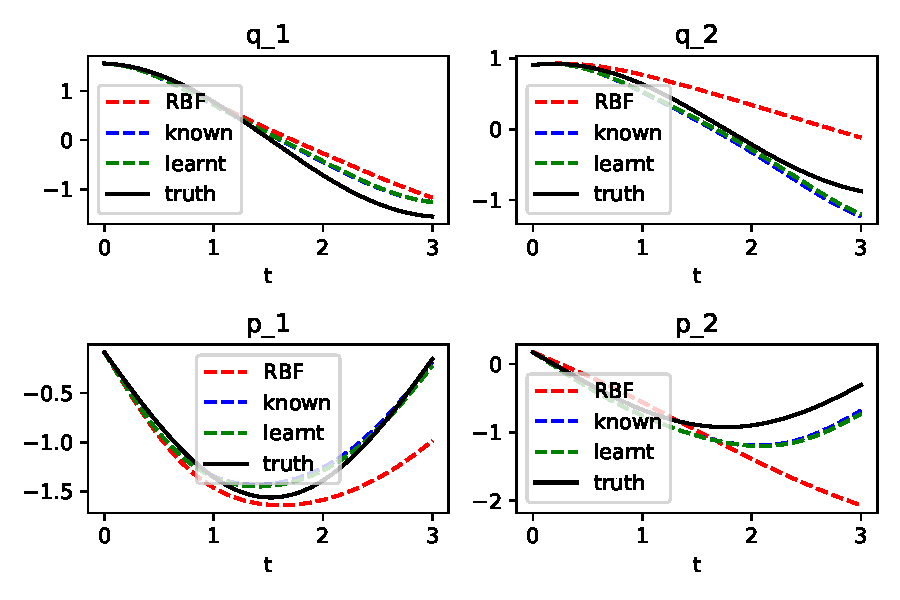
\includegraphics[width=0.8\linewidth]{../codes/figures/shm_2d_predicted.pdf}
  \centering
  \caption{Two-dimensional SHM prediction. We see the invariance kernel is very close to predict the ground truth, while RBF is again not generalising well.}
  \label{fig:shm_2d_prediction}
\end{figure}

\begin{figure}[H] 
  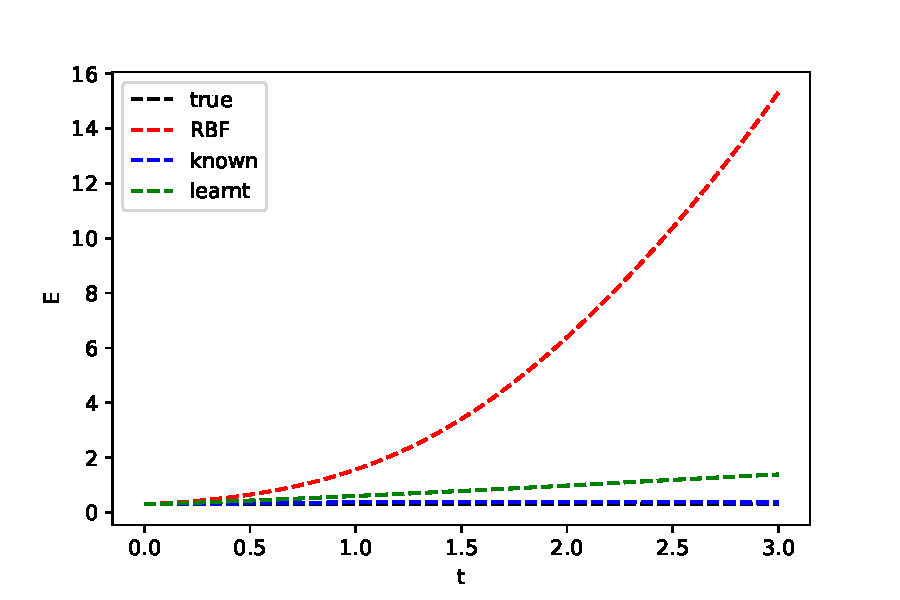
\includegraphics[width=0.8\linewidth]{../codes/figures/shm_2d_energy.pdf}
  \centering
  \caption{Two-dimensional SHM energy. The invariance kernel does very well in preserving the energy while the RBF does not respect the invariance at all.}
  \label{fig:shm_2d_energy}
\end{figure}

\begin{figure}[H] 
  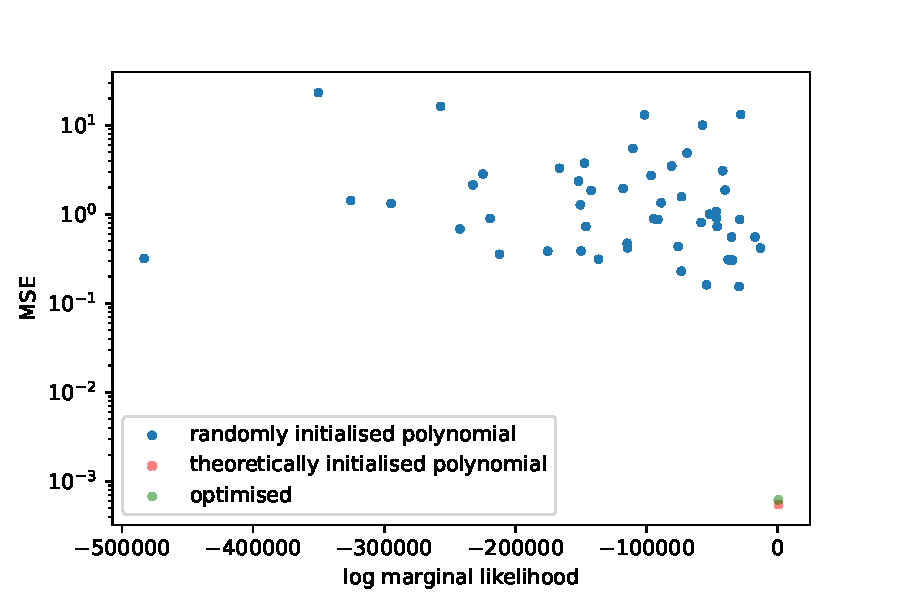
\includegraphics[width=0.8\linewidth]{../codes/figures/shm_2d_polynomial.pdf}
  \centering
  \caption{Two-dimensional SHM learnt invariance. We can see that theoretically initialised value and the freely optimised polynomial invarinace coincide and have much better MSE and marginal likelihood than the randomly initialised invariance kernel. Proving that the model is able to recognise the true invariance.}
  \label{fig:shm_2d_poly}
\end{figure}

Firstly, we can see that the invariance kernel still performs very well compared to RBF, although not as good as the 1D case as expected since higher dimensional problem is deemed to be more difficult.
We can see the learnt invariance again is almost exactly the same as the known form, which is reassuring.
Also, the conservation of energy is again pretty well obeyed.


Lastly, we confirm the above check to make sure we are indeed learning the correct invariance.
We can see the freely optimised polynoimal is exactly the same as the fixed theoretically correct value, and are much better than the randomly initialised invariance. 
We also found a Pearson correlation between log marginal likelihood and MSE of $-0.4274$ with a p value of $0.0020$, therefore, it is clear we are learning the correct invariance. 

\subsection{Nonlinear Double Pendulum}
Here we will introduce double pendulum, which is a very nonlinear system and much more complicated than all the cases we have seen before. 
It has two mass blobs $m_1$ and $m_2$ as well as two lengths for the pendulum string $\ell_1$ and $\ell_2$ as illustrated in figure \ref{fig:double_pendulum_diagram}.

\begin{figure}[H]
        \centering
        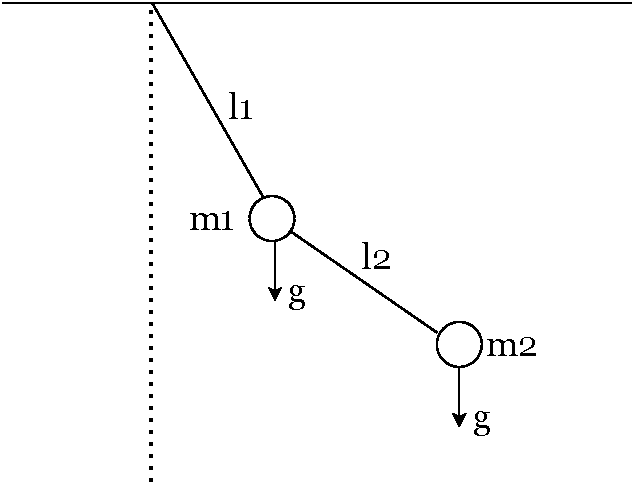
\includegraphics[width=0.4\linewidth]{../figures/doublependulum.pdf}
        \caption{Double Pendulum with much more degree of freedom, and is often an example of chaotic system.}
        \label{fig:double_pendulum_diagram}
\end{figure}

The defining equation of motion is as follows:
$$
\begin{cases}
\frac{d^2q_1}{dt^2}=\frac{-g\left(2 m_{1}+m_{2}\right) \sin q_1-m_{2} g \sin \left(q_1-2 q_2\right)-2 \sin \left(q_1-q_2\right) m_{2}\left(p_2^{2} l_{2}+p_1^{2} l_{1} \cos \left(q_1-q_2\right)\right)}{l_{1}\left(2 m_{1}+m_{2}-m_{2} \cos \left(2 q_1-2 q_2\right)\right)} \\
\frac{d^2q_2}{dt^2}=\frac{2 \sin \left(q_1-q_2\right)\left(p_1^{2} l_{1}\left(m_{1}+m_{2}\right)+g\left(m_{1}+m_{2}\right) \cos q_1+p_2{ }^{2} l_{2} m_{2} \cos \left(q_1-q_2\right)\right)}{l_{2}\left(2 m_{1}+m_{2}-m_{2} \cos \left(2 q_1-2 q_2\right)\right)}
\end{cases}
$$
As we can see, it is very complicated in term of the form.
We also have form of energy 
$$
E = -(m_1+m_2)gl_1\cos q_1-m_2gl_2\cos q_2+ \frac{m_1l^2_1p_1^2}{2}+\frac{m_2}{2}(l^2_1p_1^2+l^2_2p_2^2+2l_1l_2p_1p_2\cos(q_1-q_2))
$$
While the form is more complicated, the underlying principle to construct the invariance kernel is exactly the same as before. 
We again differentiate the energy with respect to time and set it to zero to obtain the invariance equation to obtain 
\begin{gather*}
L[\mathbf{f}]=\frac{dE}{dt} = (m_1+m_2)gl_1\sin\theta_1v_1+m_2gl_2\sin\theta_2v_2+m_1l_1^2\dot{\theta}_1a_1+\\m_2(l_1^2\dot{\theta}_1a_1+l_2^2\dot{\theta}_2a_2+l_1l_2(\dot{\theta}_2\cos(\theta_1-\theta_2)a_1+\dot{\theta}_1\cos(\theta_1-\theta_2)a_2-\dot{\theta_1}\dot{\theta_2}\sin(\theta_1-\theta_2)(v_1-v_2)))=0
\end{gather*}
The form of the invariance matrix is too cubersome to write down so it omitted here, but the derivation is as straightforward as before. 

For our experiment, with double pendulum, we have angles being between $\pm 60^\circ$ and angular velocity between $\pm 10^\circ$, so as to not make the motion too chaotic.
We also set $m_1=m_2=\ell_1=\ell_2=g=1.$
As the practice before, we initialised the polynomial coefficients at the correct theoretical value.
However, this time, because we are approximating to cubic terms only, we do not expect that initial values to perform great so we can only used the third evaluation procedure to verify it is learning the invariance along with its energy conserving performance.
We used five trajectories of length 10 time steps each.
The results are summarised in table \ref{tab:double_pendulum_performance} and predictions of trajectory in figure \ref{fig:double_pendulum_prediction} and of energy in figure \ref{fig:double_pendulum_energy}.

\begin{table}[H]
  \centering
  \begin{tabular}{l l l l}
    \hline
Method           & RBF & Known Invariance&  Learnt Invariance\\
  \hline
Log Marginal Likelihood & 783.46 & 838.41 & 869.09  \\
MSE & 0.0040 & 0.0004 & 0.0018 \\
    \hline
  \end{tabular}
  \caption{Double pendulum invariance performance. We can see the known invariance is very accurate compare to RBF, but the learnt invariance is much poorer, but still a lot better than baseline. This is likely due to the approximations made with polynomials.}
  \label{tab:double_pendulum_performance}
\end{table}

\begin{figure}[H] 
  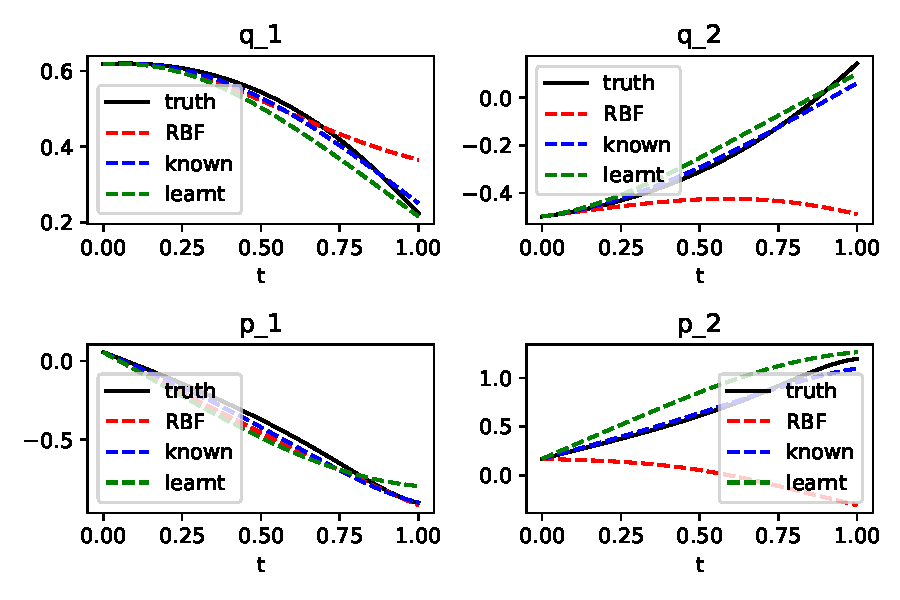
\includegraphics[width=0.8\linewidth]{../codes/figures/double_pendulum_predicted.pdf}
  \centering
  \caption{Double pendulum prediction. We can see RBF again does not generalise well, while the invariance kernels (even the learnt one) is predicting very well to the ground truth.}
  \label{fig:double_pendulum_prediction}
\end{figure}

\begin{figure}[H] 
  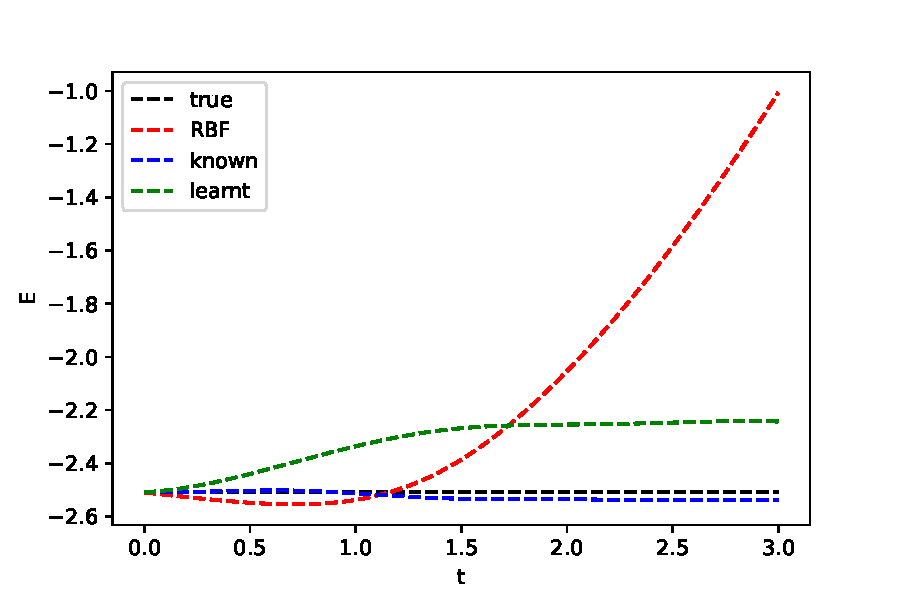
\includegraphics[width=0.8\linewidth]{../codes/figures/double_pendulum_energy.pdf}
  \centering
  \caption{Double pendulum energy. Here the known invariance is preserving the energy as expected, while the learnt invariance is slightly off but we can still tell it is trying to obey the constraints. On the other hand, the RBF completely disregards energy conservation.}
  \label{fig:double_pendulum_energy}
\end{figure}

\begin{figure}[H] 
  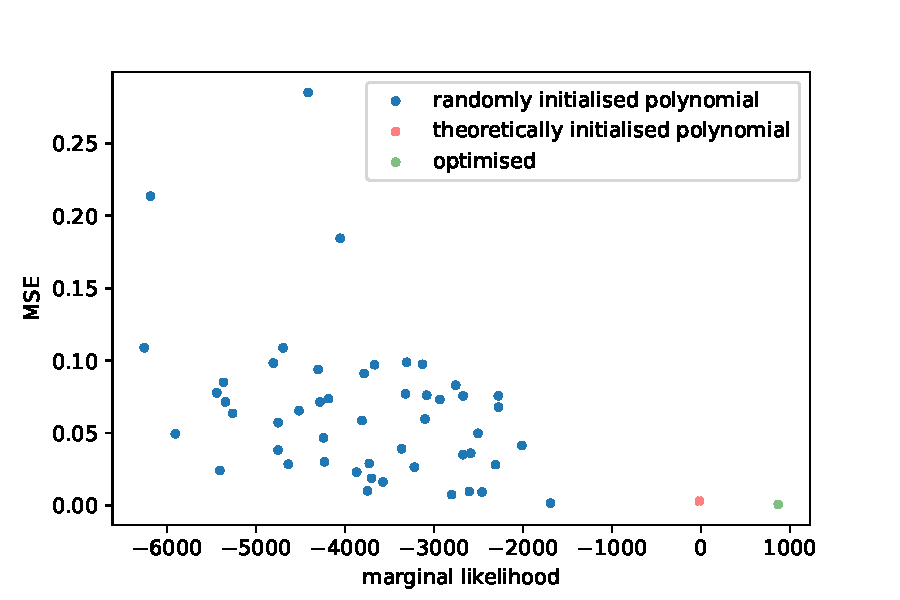
\includegraphics[width=0.8\linewidth]{../codes/figures/double_pendulum_polynomial.pdf}
  \centering
  \caption{Double Pendulum learnt invariance. Here we see the freely optimsed learnt invariance being better in both marginal likelihood and preditive performance than the theoretically approximately initialised ones as expected. Therefore, we conclude that the model is able to correctly identify the invariance.}
  \label{fig:double_pendulum_poly}
\end{figure}

Now it is interesting to obsesrve that the marginal likelihood of the learnt form is even better than known form.
This is likely due to "overfitting" of the large number of parameters from the polynomials (140 in total).
But the degree of which is not too large so we would not add regularisation which can shrink the polynomials too much so that the invariance may seem to be obeyed but it is just close to zero since the coefficients are small.
Also, we are only expanding up to the cubic term, therefore we do not expect very good learning for the invariance.
However, in our case, the approximation is fairly good, possibly due to relatively small value of $q, p$ so the polynomial approximation is good.
Nevertheless, it is clear that there is still some errors with learning invariance from figure \ref{fig:double_pendulum_energy} since it only flattens toward the end of the trajectory.

This time we found a Pearson corrletaiton of $-0.3644$ with a p-value of $0.0093$ between MSE and log marginal likelihood.
Combining with the fact that our optimised learnt kernel is better than the theortically approximately initialised kernel in both marginal likelihood and MSE, so we conclude that we have identified the correct invariance.  

\chapter{Conclusion and Future Work}
In this work, we have presented a new Gaussian Process model through an invariance kernel that is able to capture the invariance in a dynamical system and as a result, use it as an inductive bias to improve data efficiency and predictive performance in several one and two-dimensional physical systems. 
We construct this special invariance kernel by using the fact that invariances are linear transformation of the dynamics and the property of joint Gaussian distribution, and finally does the conditioning using simple Schur Complement calculation.
To learn this invariance condition, we parameterise it with polynomials and optimise the coefficients by marginal likelihood objective. 
The model is able to capture the correct invariance and recover the law of physics.
We have also demonstrated it is also robust against dissiaptive effects using a noise variable to allow "soft invariance" as well as using a latent variable to model the dissipative forces. 

In the future, there are several directions this project could evolve into.
To start off, we have demonstrated our results on relatively simple systems that could easily be sovled by first year physics undergraduate student. 
It would be interesting to see how our current model fits into the bigger picture of physical dynamical systems.
For instance, a charged particle in magnetic field still conserves energy with forces acting on it. 
Would our model able to accomdate that?
Or if the forces are time dependent, such as forced oscillation of pendulum, perhaps we need to include time as an input variable.
More generally, we are simply using the energy conservation to derive our kernel, and the form is more or less equivalent to Newton's law of motion.
There may be more complicated systems where this formulation is not sufficient.
For instance, the Lagrangian and Hamiltonian formula are much more general and could be even be extended to quantum mechanics.
For classical dynamical systems, if we want to model deformation of elastic materials or extended objects that are not point particles, this formulation may not be sufficient.
As a result, it is important to consult classical theoretical physics literature to help us understand the limitations of our models and then extend to form a more complete picture.  
In fact, Hamiltonian mechanics is the most natural way to incorporate invariance and symmetry as explained in section 2.3.
If we are able to formulate our model using Hamiltonian description, then we can easily include other symmetries such as momentum.
Another direction is to extend the partially observed system model.
We have successfully apply that in a special case of dissipative system.
However, as systems grow more complex, including a single latent dynamics may not be enough; instead, we may need to invent an latent input due to dissipative forces and derive its dyanmics by taking the time derivative.
As mentioned in section 3.4, an important and very common case is the missing input dimension problem.
If we are able to successfully recover the higher dimensional space by observing the lower dimensional space combine with the knowledge of invariance, it will be very useful in applications like 3D reconstruction.
More sophisticated inference technique will be needed such as Markov Chain Monte Carlo.


% References: modify the file refs.bib
\bibliographystyle{plainnat}
\bibliography{refs}


\clearpage
%% reset page counter and start appendix pages with A
\pagenumbering{arabic}
\renewcommand*{\thepage}{A\arabic{page}}
\appendix

\chapter{Appendix}

\section{Effect of Jitter}
Since we need a little bit of jitter to stabilise the computation of our invariance kernel as explained above, and that adding jitter is the same as adding noise to the invariance (since we are adding it on the diagonal of $LKL^T$ submatrix), we need to make sure it is not too large and too noisy, which will destroy the point of having invariance to start with. 
So we will again assess the performance in the similar way as above using different amount of jitter.
The results is shown in figure \ref{fig:vary_jitter}.

\begin{figure}[H] 
  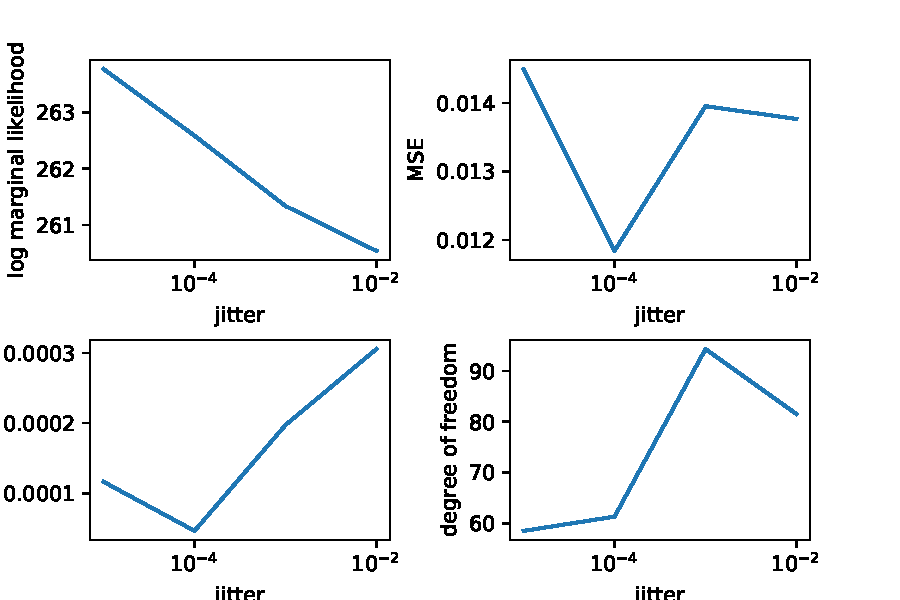
\includegraphics[width=0.8\linewidth]{../codes/figures/vary_jitter.pdf}
  \centering
  \caption{Effect of varying jitter}
  \label{fig:vary_jitter}
\end{figure}

For marginal likelihood, we see it decreases as jitter increases as expected because then the invariance is not as strong a contraint.
For MSE, we expect to see steady decrease in performance.
However, here we see a dip initially.
Again, there is not a big difference, and that the lowest jitter might not be enough to stablise the model so that the worse performance could be due to numerical instability.
We see a similar pattern in energy conservation, where we see energy consevation is not as enforced when we have noisy invariance.
Degree of freedom increases with jitter as expected since we are relaxing the constraints.
While the lower the jitter, the higher the performance should be in theory; the instability of matrix inversion and numerical errors could cause a drop in performance.
As a result,  we will also choose the smallest amount of jitter that still gives stable performance.  
Note that, in both cases of varying jitter and invariance density; all of them are much better than the RBF in performance anyways.

\end{document}
